% Options for packages loaded elsewhere
\PassOptionsToPackage{unicode}{hyperref}
\PassOptionsToPackage{hyphens}{url}
\PassOptionsToPackage{space}{xeCJK}
%
\documentclass[
  Letterpaper,
]{scrbook}

\usepackage{amsmath,amssymb}
\usepackage{iftex}
\ifPDFTeX
  \usepackage[T1]{fontenc}
  \usepackage[utf8]{inputenc}
  \usepackage{textcomp} % provide euro and other symbols
\else % if luatex or xetex
  \usepackage{unicode-math}
  \defaultfontfeatures{Scale=MatchLowercase}
  \defaultfontfeatures[\rmfamily]{Ligatures=TeX,Scale=1}
\fi
\usepackage{lmodern}
\ifPDFTeX\else  
    % xetex/luatex font selection
    \setmainfont[]{Georgia}
  \ifXeTeX
    \usepackage{xeCJK}
    \setCJKmainfont[]{STSong}
          \fi
  \ifLuaTeX
    \usepackage[]{luatexja-fontspec}
    \setmainjfont[]{STSong}
  \fi
\fi
% Use upquote if available, for straight quotes in verbatim environments
\IfFileExists{upquote.sty}{\usepackage{upquote}}{}
\IfFileExists{microtype.sty}{% use microtype if available
  \usepackage[]{microtype}
  \UseMicrotypeSet[protrusion]{basicmath} % disable protrusion for tt fonts
}{}
\makeatletter
\@ifundefined{KOMAClassName}{% if non-KOMA class
  \IfFileExists{parskip.sty}{%
    \usepackage{parskip}
  }{% else
    \setlength{\parindent}{0pt}
    \setlength{\parskip}{6pt plus 2pt minus 1pt}}
}{% if KOMA class
  \KOMAoptions{parskip=half}}
\makeatother
\usepackage{xcolor}
\usepackage[paperwidth=6in,paperheight=9in]{geometry}
\setlength{\emergencystretch}{3em} % prevent overfull lines
\setcounter{secnumdepth}{5}
% Make \paragraph and \subparagraph free-standing
\makeatletter
\ifx\paragraph\undefined\else
  \let\oldparagraph\paragraph
  \renewcommand{\paragraph}{
    \@ifstar
      \xxxParagraphStar
      \xxxParagraphNoStar
  }
  \newcommand{\xxxParagraphStar}[1]{\oldparagraph*{#1}\mbox{}}
  \newcommand{\xxxParagraphNoStar}[1]{\oldparagraph{#1}\mbox{}}
\fi
\ifx\subparagraph\undefined\else
  \let\oldsubparagraph\subparagraph
  \renewcommand{\subparagraph}{
    \@ifstar
      \xxxSubParagraphStar
      \xxxSubParagraphNoStar
  }
  \newcommand{\xxxSubParagraphStar}[1]{\oldsubparagraph*{#1}\mbox{}}
  \newcommand{\xxxSubParagraphNoStar}[1]{\oldsubparagraph{#1}\mbox{}}
\fi
\makeatother


\providecommand{\tightlist}{%
  \setlength{\itemsep}{0pt}\setlength{\parskip}{0pt}}\usepackage{longtable,booktabs,array}
\usepackage{calc} % for calculating minipage widths
% Correct order of tables after \paragraph or \subparagraph
\usepackage{etoolbox}
\makeatletter
\patchcmd\longtable{\par}{\if@noskipsec\mbox{}\fi\par}{}{}
\makeatother
% Allow footnotes in longtable head/foot
\IfFileExists{footnotehyper.sty}{\usepackage{footnotehyper}}{\usepackage{footnote}}
\makesavenoteenv{longtable}
\usepackage{graphicx}
\makeatletter
\newsavebox\pandoc@box
\newcommand*\pandocbounded[1]{% scales image to fit in text height/width
  \sbox\pandoc@box{#1}%
  \Gscale@div\@tempa{\textheight}{\dimexpr\ht\pandoc@box+\dp\pandoc@box\relax}%
  \Gscale@div\@tempb{\linewidth}{\wd\pandoc@box}%
  \ifdim\@tempb\p@<\@tempa\p@\let\@tempa\@tempb\fi% select the smaller of both
  \ifdim\@tempa\p@<\p@\scalebox{\@tempa}{\usebox\pandoc@box}%
  \else\usebox{\pandoc@box}%
  \fi%
}
% Set default figure placement to htbp
\def\fps@figure{htbp}
\makeatother

\usepackage{xeCJK}
\setCJKmainfont{STSong}
\raggedbottom
\makeatletter
\@ifpackageloaded{bookmark}{}{\usepackage{bookmark}}
\makeatother
\makeatletter
\@ifpackageloaded{caption}{}{\usepackage{caption}}
\AtBeginDocument{%
\ifdefined\contentsname
  \renewcommand*\contentsname{Table of contents}
\else
  \newcommand\contentsname{Table of contents}
\fi
\ifdefined\listfigurename
  \renewcommand*\listfigurename{List of Figures}
\else
  \newcommand\listfigurename{List of Figures}
\fi
\ifdefined\listtablename
  \renewcommand*\listtablename{List of Tables}
\else
  \newcommand\listtablename{List of Tables}
\fi
\ifdefined\figurename
  \renewcommand*\figurename{Figure}
\else
  \newcommand\figurename{Figure}
\fi
\ifdefined\tablename
  \renewcommand*\tablename{Table}
\else
  \newcommand\tablename{Table}
\fi
}
\@ifpackageloaded{float}{}{\usepackage{float}}
\floatstyle{ruled}
\@ifundefined{c@chapter}{\newfloat{codelisting}{h}{lop}}{\newfloat{codelisting}{h}{lop}[chapter]}
\floatname{codelisting}{Listing}
\newcommand*\listoflistings{\listof{codelisting}{List of Listings}}
\makeatother
\makeatletter
\makeatother
\makeatletter
\@ifpackageloaded{caption}{}{\usepackage{caption}}
\@ifpackageloaded{subcaption}{}{\usepackage{subcaption}}
\makeatother

\usepackage{bookmark}

\IfFileExists{xurl.sty}{\usepackage{xurl}}{} % add URL line breaks if available
\urlstyle{same} % disable monospaced font for URLs
\hypersetup{
  pdftitle={From Questions to Transformation},
  pdfauthor={Jian Huang},
  hidelinks,
  pdfcreator={LaTeX via pandoc}}


\title{From Questions to Transformation}
\usepackage{etoolbox}
\makeatletter
\providecommand{\subtitle}[1]{% add subtitle to \maketitle
  \apptocmd{\@title}{\par {\large #1 \par}}{}{}
}
\makeatother
\subtitle{A Practitioner's Guide to Inquiry-Based Educational Reform}
\author{Jian Huang}
\date{2025-06-10}

\begin{document}
\frontmatter
\maketitle

\renewcommand*\contentsname{Table of contents}
{
\setcounter{tocdepth}{1}
\tableofcontents
}

\mainmatter
\bookmarksetup{startatroot}

\chapter*{From Questions to
Transformation}\label{from-questions-to-transformation}
\addcontentsline{toc}{chapter}{From Questions to Transformation}

\markboth{From Questions to Transformation}{From Questions to
Transformation}

Educational transformation requires more than good intentions and
incremental adjustments---it demands systematic approaches that
fundamentally shift how students and teachers engage with learning. The
Three Questions, Three Explorations methodology represents a
comprehensive framework for moving beyond traditional pedagogical models
toward inquiry-driven classrooms where students develop critical
thinking capabilities and genuine intellectual curiosity. This approach
challenges the comfortable patterns of information delivery that have
dominated education for generations, instead positioning questioning,
exploration, and discovery as the central drivers of learning.

Successful implementation of inquiry-based reform hinges on strategic
top-level design, consensus building among stakeholders, and sustained
leadership commitment. Drawing from case studies across China's
educational landscape and regional reform initiatives, this guide
provides educational leaders with practical tools for navigating the
complex transition from pilot programs to system-wide transformation.
Rather than offering theoretical abstractions, each chapter presents
actionable strategies for overcoming common implementation pitfalls,
developing teacher capacity, and creating evaluation systems that
support rather than undermine innovative practices. The goal is not
simply to adopt new teaching methods, but to fundamentally restructure
educational environments where both students and educators become active
participants in the learning process.

\bookmarksetup{startatroot}

\chapter*{Introduction}\label{introduction}
\addcontentsline{toc}{chapter}{Introduction}

\markboth{Introduction}{Introduction}

This book explores the transformative potential of inquiry-based
learning approaches within educational systems, with a particular focus
on implementation strategies and systemic change. Throughout the
following chapters, we examine the philosophical foundations, practical
methodologies, and leadership requirements for successfully
transitioning from traditional teaching paradigms to more dynamic,
student-centered learning environments.

The inquiry-based model presented in this book, particularly the ``Three
Questions, Three Explorations'' approach, represents a significant
departure from conventional educational practices. Rather than
positioning students as passive recipients of knowledge, this framework
empowers learners to develop critical thinking skills through guided
questioning and exploration.

As educational systems worldwide seek to prepare students for
increasingly complex futures, the methods described in this book offer
pathways for meaningful reform that goes beyond superficial changes to
address the fundamental nature of teaching and learning.

\section*{Structure of the Book}\label{structure-of-the-book}
\addcontentsline{toc}{section}{Structure of the Book}

\markright{Structure of the Book}

The book begins by establishing theoretical foundations before moving
into practical implementation strategies, leadership considerations, and
sustainability approaches. Each chapter builds upon previous content
while offering distinct insights into particular aspects of educational
transformation.

\section*{Who Should Read This Book}\label{who-should-read-this-book}
\addcontentsline{toc}{section}{Who Should Read This Book}

\markright{Who Should Read This Book}

This resource is designed for educational leaders, policymakers,
curriculum developers, and teachers interested in meaningful educational
reform. The principles discussed are applicable across various
educational contexts, though specific implementation strategies may need
adaptation for different cultural and institutional settings.

\bookmarksetup{startatroot}

\chapter{Foundations of Educational
Transformation}\label{foundations-of-educational-transformation}

\section{The Imperative for Change}\label{the-imperative-for-change}

Educational systems worldwide face an unprecedented challenge: preparing
students for a rapidly evolving world while operating within structures
designed for an industrial age. The traditional model of
education---characterized by passive information transmission,
standardized curricula, and teacher-centered instruction---increasingly
fails to develop the critical thinking, adaptability, and collaborative
skills essential for 21st-century success.

This foundational chapter establishes the philosophical and theoretical
groundwork for a fundamental shift toward inquiry-based learning,
examining why transformation is necessary, what principles should guide
it, and how educators can build sustainable change that truly serves
student development.

\section{The Limitations of Traditional Educational
Paradigms}\label{the-limitations-of-traditional-educational-paradigms}

\subsection{The Banking Model of
Education}\label{the-banking-model-of-education}

Paulo Freire's critique of the ``banking model'' of education remains
strikingly relevant today. In this paradigm, teachers deposit knowledge
into passive student receptacles, creating what he termed a ``culture of
silence'' where learners become mere consumers rather than creators of
knowledge. This approach fundamentally misunderstands the nature of
learning and human development.

Traditional education typically operates on several problematic
assumptions:

\textbf{Knowledge as Static Information}: The belief that education
primarily involves transferring predetermined content from teacher to
student ignores the dynamic, constructed nature of understanding. True
learning requires active engagement with ideas, not passive absorption.

\textbf{One-Size-Fits-All Delivery}: Standardized approaches assume all
students learn identically, ignoring diverse learning styles, cultural
backgrounds, and individual developmental trajectories. This leads to
systemic inequities and missed potential.

\textbf{Teacher as Sole Authority}: Positioning teachers as the
exclusive source of valid knowledge stifles student curiosity and
independent thinking. It creates dependency rather than developing
autonomous learners.

\textbf{Compliance Over Curiosity}: Traditional systems often prioritize
behavioral compliance and correct answers over questioning, exploration,
and creative problem-solving---the very skills most valued in
contemporary society.

\subsection{The Mismatch with Contemporary
Needs}\label{the-mismatch-with-contemporary-needs}

Modern challenges require fundamentally different competencies than
those developed through traditional education. Today's students must
navigate information abundance rather than scarcity, collaborate across
diverse networks, adapt to rapid technological change, and solve
complex, interdisciplinary problems. These demands require:

\begin{itemize}
\tightlist
\item
  \textbf{Critical thinking skills} to evaluate information quality and
  bias
\item
  \textbf{Collaborative abilities} to work effectively in diverse teams
\item
  \textbf{Adaptability} to thrive amid constant change
\item
  \textbf{Creative problem-solving} to address novel challenges
\item
  \textbf{Self-directed learning} to pursue lifelong education
\item
  \textbf{Systems thinking} to understand complex interconnections
\end{itemize}

Traditional educational approaches, focused on content delivery and
standardized assessment, inadequately develop these essential
capabilities.

\section{Philosophical Foundations of Inquiry-Based
Learning}\label{philosophical-foundations-of-inquiry-based-learning}

\subsection{Constructivist Learning
Theory}\label{constructivist-learning-theory}

Inquiry-based education draws heavily from constructivist learning
theory, which posits that learners actively construct understanding
through experience and reflection rather than passively receiving
information. This perspective, influenced by Jean Piaget's developmental
psychology and Lev Vygotsky's social learning theory, emphasizes several
key principles:

\textbf{Active Knowledge Construction}: Students build understanding by
connecting new information to existing knowledge structures, requiring
active engagement with content rather than passive reception.

\textbf{Social Learning}: Knowledge develops through interaction with
others, making collaborative inquiry and discussion essential components
of effective education.

\textbf{Zone of Proximal Development}: Optimal learning occurs when
students work slightly beyond their current ability level with
appropriate support, suggesting the importance of scaffolded inquiry
experiences.

\textbf{Metacognitive Awareness}: Students learn more effectively when
they understand their own thinking processes, making reflection and
self-assessment integral to inquiry-based approaches.

\subsection{Dewey's Experiential
Learning}\label{deweys-experiential-learning}

John Dewey's educational philosophy provides crucial foundations for
inquiry-based learning. His emphasis on ``learning by doing'' and
connecting education to real-world experience aligns directly with
inquiry-based principles. Dewey argued that genuine learning occurs
through:

\textbf{Problem-Solving Experiences}: Students develop understanding by
grappling with authentic problems that connect to their lives and
interests.

\textbf{Reflective Thinking}: Experience alone is insufficient; students
must reflect on their experiences to extract meaningful learning.

\textbf{Democratic Participation}: Education should prepare students for
active citizenship, requiring opportunities to practice democratic
decision-making and collaborative problem-solving.

\textbf{Continuous Reconstruction}: Learning involves continuously
reconstructing experience and understanding, emphasizing growth and
adaptation over static knowledge acquisition.

\subsection{The Socratic Tradition}\label{the-socratic-tradition}

The inquiry-based approach also draws from the Socratic tradition of
education, which emphasizes questioning as the primary tool for
developing understanding. Socratic methodology involves:

\textbf{Strategic Questioning}: Using carefully crafted questions to
guide students toward deeper understanding rather than providing direct
answers.

\textbf{Intellectual Humility}: Acknowledging the limits of current
knowledge and maintaining openness to new insights and perspectives.

\textbf{Collaborative Inquiry}: Engaging in shared exploration of
complex questions rather than competitive demonstration of knowledge.

\textbf{Process Over Product}: Valuing the thinking process and
questioning journey as much as specific conclusions or answers.

\section{Core Principles of Educational
Transformation}\label{core-principles-of-educational-transformation}

\subsection{Principle 1: Student-Centered
Learning}\label{principle-1-student-centered-learning}

Effective educational transformation places students at the center of
the learning process. This involves:

\textbf{Honoring Student Voice}: Recognizing students as partners in
their education rather than passive recipients, incorporating their
questions, interests, and perspectives into curriculum design.

\textbf{Differentiated Instruction}: Adapting teaching methods and
content to accommodate diverse learning styles, abilities, and cultural
backgrounds.

\textbf{Choice and Autonomy}: Providing students with meaningful choices
about their learning, fostering intrinsic motivation and ownership.

\textbf{Authentic Assessment}: Using assessment methods that capture
genuine learning and growth rather than mere information recall.

\subsection{Principle 2: Inquiry as the Engine of
Learning}\label{principle-2-inquiry-as-the-engine-of-learning}

Inquiry serves as the primary mechanism for deep learning and
understanding:

\textbf{Question-Driven Curriculum}: Organizing learning around
compelling questions rather than predetermined content sequences.

\textbf{Scientific Thinking}: Teaching students to form hypotheses,
gather evidence, analyze data, and draw conclusions across all subject
areas.

\textbf{Multiple Perspectives}: Encouraging students to examine issues
from various viewpoints and consider alternative explanations.

\textbf{Iterative Learning}: Embracing learning as a cyclical process of
questioning, investigating, reflecting, and questioning anew.

\subsection{Principle 3: Collaborative Knowledge
Construction}\label{principle-3-collaborative-knowledge-construction}

Learning occurs most effectively in social contexts where students can
share ideas, challenge assumptions, and build understanding together:

\textbf{Peer Learning}: Structuring opportunities for students to learn
from and with each other through discussion, collaboration, and peer
feedback.

\textbf{Community Connections}: Linking classroom learning to broader
community issues and resources, making education relevant and
purposeful.

\textbf{Cultural Responsiveness}: Honoring and incorporating diverse
cultural knowledge and ways of knowing into the learning process.

\textbf{Shared Responsibility}: Distributing responsibility for learning
across students, teachers, and community members rather than placing it
solely on individual students.

\subsection{Principle 4: Reflective
Practice}\label{principle-4-reflective-practice}

Both students and educators must engage in ongoing reflection to support
continuous improvement:

\textbf{Metacognitive Development}: Teaching students to think about
their thinking, understanding their learning processes and strategies.

\textbf{Professional Learning Communities}: Creating structures for
educators to collaborate, share practices, and engage in collective
inquiry about teaching and learning.

\textbf{Action Research}: Encouraging educators to systematically study
their own practice and its impact on student learning.

\textbf{Continuous Improvement}: Embracing change and adaptation as
essential components of effective education rather than obstacles to
overcome.

\section{The Neuroscience of
Learning}\label{the-neuroscience-of-learning}

Recent advances in neuroscience provide compelling support for
inquiry-based educational approaches. Key findings include:

\subsection{Brain Plasticity and
Growth}\label{brain-plasticity-and-growth}

The brain's capacity for change throughout life supports the importance
of challenging, engaging learning experiences. Inquiry-based approaches
promote neuroplasticity by:

\begin{itemize}
\tightlist
\item
  Creating rich, multi-sensory learning environments
\item
  Encouraging novel problem-solving experiences
\item
  Supporting emotional engagement with learning
\item
  Providing opportunities for reflection and consolidation
\end{itemize}

\subsection{Memory and Understanding}\label{memory-and-understanding}

Research on memory formation reveals that deep, lasting learning
requires:

\textbf{Elaborative Processing}: Connecting new information to existing
knowledge networks rather than rote memorization.

\textbf{Distributed Practice}: Spacing learning experiences over time
rather than massing them together.

\textbf{Retrieval Practice}: Actively recalling information and applying
it in new contexts rather than passive review.

\textbf{Interleaving}: Mixing different types of problems and concepts
rather than practicing them in isolation.

Inquiry-based approaches naturally incorporate these effective learning
strategies.

\subsection{Motivation and Engagement}\label{motivation-and-engagement}

Neuroscientific research on motivation aligns closely with inquiry-based
principles:

\textbf{Intrinsic Motivation}: The brain's reward systems respond more
strongly to internally motivated activities than externally imposed
requirements.

\textbf{Curiosity and Exploration}: The brain is naturally wired to seek
novelty and explore unknown territories, making inquiry a fundamentally
human activity.

\textbf{Social Connection}: Mirror neurons and social brain networks
highlight the importance of collaborative learning experiences.

\textbf{Growth Mindset}: Understanding that abilities can be developed
through effort and practice, supported by neuroplasticity research,
enhances student resilience and achievement.

\section{Addressing Common Concerns and
Misconceptions}\label{addressing-common-concerns-and-misconceptions}

\subsection{``Students Need Content Knowledge
First''}\label{students-need-content-knowledge-first}

Critics often argue that inquiry-based approaches neglect essential
content knowledge in favor of process skills. This false dichotomy
misunderstands how inquiry-based learning operates. Effective
inquiry-based education:

\begin{itemize}
\tightlist
\item
  Uses content knowledge as a tool for investigation rather than an end
  in itself
\item
  Develops deeper, more transferable understanding of content through
  active engagement
\item
  Integrates content learning with skill development rather than
  treating them separately
\item
  Recognizes that knowledge and thinking skills develop together, not
  sequentially
\end{itemize}

\subsection{``Inquiry Takes Too Much
Time''}\label{inquiry-takes-too-much-time}

Concerns about curriculum coverage often arise when considering
inquiry-based approaches. However, research demonstrates that:

\begin{itemize}
\tightlist
\item
  Deep learning of fewer concepts leads to better long-term retention
  and transfer than surface coverage of many topics
\item
  Students develop more efficient learning strategies through inquiry
  experiences
\item
  Integrated, thematic approaches can address multiple curriculum
  objectives simultaneously
\item
  Students become more self-directed learners, reducing
  teacher-dependent instruction time
\end{itemize}

\subsection{``Not All Students Can Handle
Inquiry''}\label{not-all-students-can-handle-inquiry}

Some educators worry that inquiry-based approaches work only for
high-achieving students. Evidence suggests otherwise:

\begin{itemize}
\tightlist
\item
  All students have natural curiosity and questioning abilities that can
  be developed
\item
  Struggling students often thrive when given agency and choice in their
  learning
\item
  Inquiry-based approaches can be scaffolded to support learners at
  different levels
\item
  Students from diverse backgrounds bring valuable perspectives to
  inquiry experiences
\end{itemize}

\section{Building the Foundation for
Change}\label{building-the-foundation-for-change}

Educational transformation requires careful attention to foundational
elements that support sustainable change:

\subsection{Cultural Shift}\label{cultural-shift}

Moving from traditional to inquiry-based education requires fundamental
cultural change within educational institutions. This involves:

\textbf{Shared Vision}: Developing collective understanding of why
change is necessary and what success looks like.

\textbf{Risk-Taking Culture}: Creating environments where
experimentation and learning from failure are valued.

\textbf{Collaborative Norms}: Establishing expectations for professional
collaboration and shared responsibility.

\textbf{Student Voice}: Systematically incorporating student
perspectives into decision-making processes.

\subsection{Structural Alignment}\label{structural-alignment}

Educational structures must align with inquiry-based principles:

\textbf{Flexible Scheduling}: Allowing time for in-depth investigation
and authentic assessment.

\textbf{Physical Spaces}: Designing learning environments that support
collaboration, investigation, and multiple ways of working.

\textbf{Assessment Systems}: Developing evaluation methods that capture
the full range of student learning and growth.

\textbf{Professional Development}: Providing ongoing support for
educator learning and growth.

\subsection{Leadership Support}\label{leadership-support}

Effective transformation requires committed leadership at all levels:

\textbf{Vision Communication}: Clearly articulating the purpose and
benefits of inquiry-based education.

\textbf{Resource Allocation}: Providing necessary time, materials, and
support for implementation.

\textbf{Barrier Removal}: Identifying and addressing obstacles to
effective practice.

\textbf{Celebration of Success}: Recognizing and sharing examples of
effective inquiry-based learning.

\section{Conclusion: The Path
Forward}\label{conclusion-the-path-forward}

The foundations of educational transformation rest on a fundamental
shift in how we understand learning, teaching, and the purpose of
education itself. Moving from traditional, teacher-centered approaches
to inquiry-based, student-centered methods requires more than
superficial changes in classroom techniques---it demands a
reconceptualization of education as a collaborative, investigative, and
transformative process.

This transformation is not merely desirable but essential for preparing
students to thrive in an increasingly complex and rapidly changing
world. The philosophical foundations, neuroscientific evidence, and
practical principles outlined in this chapter provide the groundwork for
implementing inquiry-based approaches that honor student potential,
develop essential 21st-century skills, and create more equitable and
engaging educational experiences.

The journey toward educational transformation begins with understanding
these foundations and committing to the deep, systemic change they
require. Subsequent chapters will explore the practical strategies,
implementation approaches, and support systems necessary to translate
these principles into transformative educational practice.

As we embark on this transformation, we must remember that education is
fundamentally about human development and potential. Inquiry-based
approaches honor the natural curiosity, creativity, and capacity for
growth that all students possess, creating learning environments where
every individual can flourish and contribute to our collective
understanding and progress.

\bookmarksetup{startatroot}

\chapter{Building Consensus and Shared
Vision}\label{building-consensus-and-shared-vision}

\section{Introduction: The Imperative of Collective
Commitment}\label{introduction-the-imperative-of-collective-commitment}

Educational transformation cannot succeed as a solitary endeavor. While
individual educators may implement innovative practices within their
classrooms, sustainable systemic change requires what the Chinese
educational reform literature describes as \emph{gongshengli} (共识力)
--- consensus-building power. This chapter examines the critical
processes through which educational communities develop unified goals,
reduce resistance to change, and create collaborative environments where
administrators, teachers, students, and community members work together
toward common educational objectives.

The challenge of building consensus in educational settings is
particularly acute because schools function as complex adaptive systems
where multiple stakeholders hold varying perspectives on learning,
teaching, and institutional purpose. Teachers bring professional
experience and pedagogical beliefs developed over years of practice.
Administrators balance educational vision with practical constraints of
budgets, regulations, and political pressures. Parents and community
members contribute expectations shaped by their own educational
experiences and cultural values. Students themselves, often overlooked
in reform conversations, possess insights about learning that can either
support or undermine transformational efforts.

Successfully navigating these diverse perspectives requires more than
simple communication or superficial agreement. It demands what
educational theorist Michael Fullan describes as ``coherence-making''
--- the systematic development of shared understanding that transcends
individual positions and creates genuine collective commitment to
change. This process forms the foundation upon which all subsequent
reform efforts must build.

\section{Understanding Resistance as
Information}\label{understanding-resistance-as-information}

Before exploring consensus-building strategies, we must recognize that
resistance to educational change often contains valuable information
about institutional realities and stakeholder concerns. Rather than
viewing resistance as an obstacle to overcome, effective change leaders
approach it as a diagnostic tool that reveals underlying tensions,
unaddressed needs, and potential implementation challenges.

Resistance typically manifests in several forms within educational
contexts. \emph{Cognitive resistance} emerges when stakeholders question
the theoretical foundation or empirical evidence supporting proposed
changes. Teachers may ask whether inquiry-based approaches actually
improve learning outcomes compared to direct instruction methods they
have successfully employed for years. This form of resistance often
reflects genuine intellectual engagement with reform proposals and can
lead to more robust implementation strategies when addressed
thoughtfully.

\emph{Emotional resistance} develops when changes threaten professional
identity or personal security. A veteran teacher who has built expertise
in lecture-based instruction may experience anxiety about adopting
inquiry-based methods that require fundamentally different skills. This
resistance is often mischaracterized as mere stubbornness, but it
actually reflects legitimate concerns about professional competence and
effectiveness during transition periods.

\emph{Practical resistance} arises from resource constraints, time
limitations, or structural barriers that make implementation difficult
regardless of theoretical commitment. Teachers may enthusiastically
support inquiry-based learning while simultaneously recognizing that
their current class sizes, physical spaces, or assessment requirements
make such approaches impractical without systemic support.

\emph{Cultural resistance} reflects deeper disagreements about
educational purpose and values. Community members who view education
primarily as knowledge transmission may question approaches that
emphasize student questioning and exploration over content mastery.
These tensions often reveal fundamental philosophical differences that
require careful negotiation rather than simple persuasion.

Effective consensus-building acknowledges each form of resistance as
legitimate while working to address underlying concerns through
collaborative problem-solving. This approach transforms potential
adversaries into partners in developing solutions that honor stakeholder
perspectives while advancing reform objectives.

\section{Creating Conditions for Productive
Dialogue}\label{creating-conditions-for-productive-dialogue}

Meaningful consensus emerges through structured dialogue processes that
create psychological safety, encourage diverse perspectives, and focus
on shared values rather than immediate tactical disagreements. The
Chinese educational reform experience emphasizes the importance of
\emph{xuexixing zuzhii} (学习型组织) --- learning organizations --- that
prioritize collective inquiry over individual advocacy.

Establishing psychological safety requires leaders to demonstrate
genuine openness to criticism and alternative viewpoints. Teachers must
feel confident that expressing concerns about reform proposals will not
result in professional retaliation or marginalization. This means
creating formal mechanisms for dissent and ensuring that critical voices
are heard and respected rather than dismissed or ignored.

The physical and temporal structures of dialogue also matter
significantly. Brief faculty meetings dominated by administrative
announcements provide insufficient space for meaningful conversation
about complex educational changes. Effective consensus-building requires
dedicated time and appropriate venues where stakeholders can engage in
substantive discussion without the pressure of immediate
decision-making.

One particularly effective approach involves what organizational
psychologist Edgar Schein calls ``humble inquiry'' --- questioning that
demonstrates genuine curiosity about stakeholder perspectives rather
than leading toward predetermined conclusions. Instead of asking ``How
can we convince teachers to adopt inquiry-based methods?'' leaders might
ask ``What concerns do teachers have about inquiry-based approaches, and
what would need to be true for these methods to work effectively in our
context?''

This shift from advocacy to inquiry fundamentally changes the dynamics
of reform conversations. Rather than defending predetermined positions,
participants collaborate in exploring possibilities and identifying
solutions that address collective concerns while advancing shared
educational goals.

\section{Identifying and Leveraging Shared
Values}\label{identifying-and-leveraging-shared-values}

While stakeholders may disagree about specific educational practices,
they often share deeper commitments to student welfare, professional
growth, and institutional excellence. Effective consensus-building
identifies these shared values and uses them as anchoring points for
reform discussions.

Most educators, regardless of their pedagogical preferences, want
students to develop critical thinking skills, maintain engagement with
learning, and achieve academic success. Parents typically desire
educational experiences that prepare their children for future
opportunities while supporting their personal development. Community
members generally value schools that contribute to local economic
vitality and social cohesion.

These shared values provide common ground for exploring how
inquiry-based approaches might serve collective interests. Rather than
beginning with debates about specific teaching methods,
consensus-building processes can start by examining whether current
educational practices effectively serve these shared commitments. This
approach often reveals gaps between stated values and actual outcomes
that create openings for considering alternative approaches.

The process of values clarification also helps distinguish between
negotiable and non-negotiable aspects of reform proposals. While
specific implementation strategies may require adaptation to local
contexts, core principles of inquiry-based learning --- such as
respecting student intelligence and fostering active engagement with
ideas --- often align closely with stakeholder values once these
connections are made explicit.

\section{Developing Collective
Efficacy}\label{developing-collective-efficacy}

Consensus alone is insufficient for sustaining educational
transformation. Stakeholders must also develop confidence in their
collective ability to implement proposed changes successfully.
Educational researcher John Hattie's meta-analyses consistently identify
collective teacher efficacy as one of the most powerful factors
influencing student achievement, with effect sizes substantially larger
than most individual teaching strategies.

Collective efficacy develops through shared experiences of success that
demonstrate the group's capacity to overcome challenges and achieve
meaningful goals. This suggests that consensus-building processes should
include opportunities for stakeholders to work together on manageable
projects that build confidence while advancing reform objectives.

Pilot programs serve this function particularly well when designed as
collaborative learning experiences rather than simple implementation
tests. When small groups of teachers work together to develop and refine
inquiry-based lessons, they simultaneously build skills, strengthen
relationships, and generate evidence about what works in their specific
context. Success with these limited initiatives creates momentum and
confidence for broader implementation.

The role of external support in building collective efficacy cannot be
understated. As evidenced in the Jilin Province reform experiences
described in the source materials, bringing in experts who can provide
technical assistance while validating local efforts helps stakeholders
develop confidence in their ability to implement sophisticated changes.
However, this support must be offered in ways that build internal
capacity rather than creating dependency on external expertise.

\section{Managing the Pace of Consensus
Development}\label{managing-the-pace-of-consensus-development}

Educational leaders often face pressure to achieve consensus quickly in
order to begin implementation, but rushed consensus-building typically
produces superficial agreement that dissolves under the stress of actual
change. Sustainable consensus requires sufficient time for stakeholders
to process new information, explore implications, and work through
concerns.

The Chinese concept of \emph{chixu tuijin} (持续推进) --- persistent
advancement --- suggests a approach that balances urgency with patience.
Reform leaders maintain consistent pressure toward change while allowing
adequate time for consensus to develop authentically. This requires
distinguishing between appropriate timelines for different aspects of
the change process.

Initial awareness-building and values clarification may occur relatively
quickly, particularly when facilitated by skilled leaders who can help
stakeholders recognize existing alignment. However, developing specific
implementation strategies and building collective efficacy typically
requires months or even years of sustained engagement.

The temptation to shortcut this process by imposing changes through
administrative authority almost invariably backfires. While compliance
may be achieved temporarily, genuine implementation requires the kind of
deep commitment that emerges only through authentic consensus-building
processes.

\section{Communication Strategies for Diverse
Audiences}\label{communication-strategies-for-diverse-audiences}

Different stakeholders require different types of information and
engagement to develop commitment to educational reform. Effective
consensus-building recognizes these differences and tailors
communication strategies accordingly while maintaining message
consistency.

Teachers typically respond well to evidence-based arguments that include
research findings, implementation examples from similar contexts, and
opportunities to observe or experience inquiry-based approaches
firsthand. They often appreciate detailed discussions of pedagogical
theory and practical implementation strategies that acknowledge the
complexity of classroom management and student engagement.

Administrators may focus more heavily on alignment with district
priorities, resource requirements, and potential impacts on standardized
test performance. They often need information about implementation
timelines, professional development costs, and strategies for managing
community relations during transition periods.

Parents and community members may be most interested in understanding
how proposed changes will affect their children's educational
experiences and future opportunities. They often appreciate
straightforward explanations of research findings, concrete examples of
student learning, and opportunities to observe inquiry-based approaches
in action.

Students themselves deserve age-appropriate explanations of proposed
changes and opportunities to provide input about their learning
preferences and concerns. While their formal decision-making power may
be limited, their perspectives often reveal important implementation
considerations that adults might overlook.

The key principle underlying all these communication strategies is
transparency about both benefits and challenges of proposed changes.
Stakeholders develop greater trust and commitment when leaders
acknowledge difficulties honestly rather than overselling reform
proposals or minimizing implementation challenges.

\section{Institutionalizing Consensus Through Structural
Changes}\label{institutionalizing-consensus-through-structural-changes}

While consensus initially develops through dialogue and
relationship-building, it must be reinforced through institutional
structures that embed shared commitments into organizational routines
and decision-making processes. Without such institutionalization,
consensus remains fragile and may deteriorate when key leaders leave or
external pressures mount.

Governance structures provide one important mechanism for
institutionalizing consensus. When teachers, parents, and community
members have formal roles in educational decision-making, they develop
stronger ownership of reform initiatives and greater commitment to their
success. However, these structures must involve genuine power-sharing
rather than superficial consultation if they are to strengthen consensus
effectively.

Professional development systems offer another avenue for embedding
consensus in institutional practice. When teachers collaborate regularly
in examining student work, refining instructional strategies, and
solving implementation challenges, they continuously recreate and
strengthen their shared commitment to inquiry-based approaches. These
ongoing interactions prevent consensus from becoming static and help it
evolve in response to new learning and changing circumstances.

Evaluation and accountability systems also play crucial roles in
sustaining consensus by focusing attention on outcomes that matter to
stakeholders. When assessment practices emphasize the kind of deep
learning that inquiry-based approaches promote, they reinforce
stakeholder commitment to these methods. Conversely, when accountability
systems reward only traditional measures of academic achievement, they
undermine consensus by creating tensions between stated values and
actual incentives.

\section{Conclusion: Consensus as Foundation for
Transformation}\label{conclusion-consensus-as-foundation-for-transformation}

Building consensus and shared vision represents foundational work that
enables all subsequent aspects of educational transformation. Without
genuine stakeholder commitment, even the most sophisticated reform
strategies will fail to achieve lasting change. However, when
educational communities develop authentic shared understanding and
collective commitment, they create the conditions necessary for
sustained innovation and improvement.

The process of consensus-building is itself educational, developing
stakeholder capacity for collaborative problem-solving, shared
decision-making, and continuous improvement. These capabilities serve
educational organizations well beyond any particular reform initiative,
creating adaptive capacity that enables ongoing evolution in response to
changing student needs and social contexts.

As we will explore in Chapter 3, effective consensus provides the
foundation for strategic top-level design that translates shared vision
into coherent action plans. Without this foundation, even the most
carefully crafted implementation strategies will struggle to achieve
their intended outcomes. With it, educational communities position
themselves to undertake the systematic transformation necessary to serve
all students effectively in an increasingly complex and dynamic world.

\bookmarksetup{startatroot}

\chapter{Strategic Top-Level Design}\label{strategic-top-level-design}

\section{Introduction}\label{introduction-1}

Strategic top-level design represents the architectural foundation upon
which successful educational transformation rests. Unlike piecemeal
reforms that address symptoms rather than systemic issues, strategic
design begins with a clear vision of desired outcomes and works
backwards through methodical planning to create coherent, sustainable
change pathways. This approach, fundamental to the inquiry-based
learning revolution, demands that educational leaders think like systems
architects rather than incremental managers.

The Chinese educational reform documents emphasize a critical principle:
``改思维,以终为始'' (gǎi sīwéi, yǐ zhōng wéi shǐ) --- transform
thinking by beginning with the end in mind. This concept, borrowed from
Stephen Covey's influential work but deeply rooted in traditional
Chinese strategic thought, forms the cornerstone of effective
educational design. Rather than asking ``what can we change?'' strategic
designers ask ``what must our graduates become?'' and design backwards
from that vision.

Strategic top-level design differs fundamentally from traditional reform
approaches in its scope, coherence, and temporal perspective. Where
conventional reforms often address isolated problems with isolated
solutions, strategic design creates integrated systems where each
component reinforces others. This integration proves particularly
crucial in inquiry-based learning implementations, where classroom
practices, assessment systems, teacher development, and institutional
culture must align to support student questioning and exploration.

\section{The Architecture of Educational
Vision}\label{the-architecture-of-educational-vision}

Effective strategic design begins with what we might call ``vision
architecture'' --- the systematic construction of clear, measurable, and
inspiring educational outcomes. This process requires educational
leaders to move beyond vague aspirations like ``improving student
learning'' toward specific competencies, mindsets, and capabilities that
define successful graduates.

Vision architecture in inquiry-based systems centers on developing
students who can formulate meaningful questions, pursue evidence-based
investigations, and construct knowledge through exploration rather than
passive reception. This vision must be articulated with sufficient
specificity that teachers, administrators, parents, and students
themselves can recognize progress toward its achievement.

The Chinese reform experiences demonstrate that effective vision
architecture operates at multiple levels simultaneously. At the broadest
level, leaders must articulate how inquiry-based learning serves
societal needs for creative, critical thinkers capable of addressing
complex challenges. At the institutional level, they must specify how
inquiry approaches will transform school culture, classroom dynamics,
and student-teacher relationships. At the individual level, they must
describe the specific skills, attitudes, and knowledge that
inquiry-based graduates will possess.

Consider the example of Xiaxia No.~1 High School, which developed its
``Three Questions, Three Explorations'' model through careful vision
architecture. School leaders began by envisioning graduates who could
independently identify important questions, systematically investigate
complex problems, and communicate findings effectively. Working
backwards from this vision, they designed classroom protocols, teacher
development programs, and assessment systems that incrementally built
these capabilities throughout students' educational journey.

This backwards design process reveals a fundamental principle of
strategic architecture: coherence emerges from alignment rather than
accumulation. Rather than adding inquiry-based practices to existing
traditional structures, effective design rebuilds educational systems
around inquiry principles. This rebuilding requires leaders to examine
every aspect of schooling --- from curriculum sequencing to physical
space design --- through the lens of their ultimate vision.

\pandocbounded{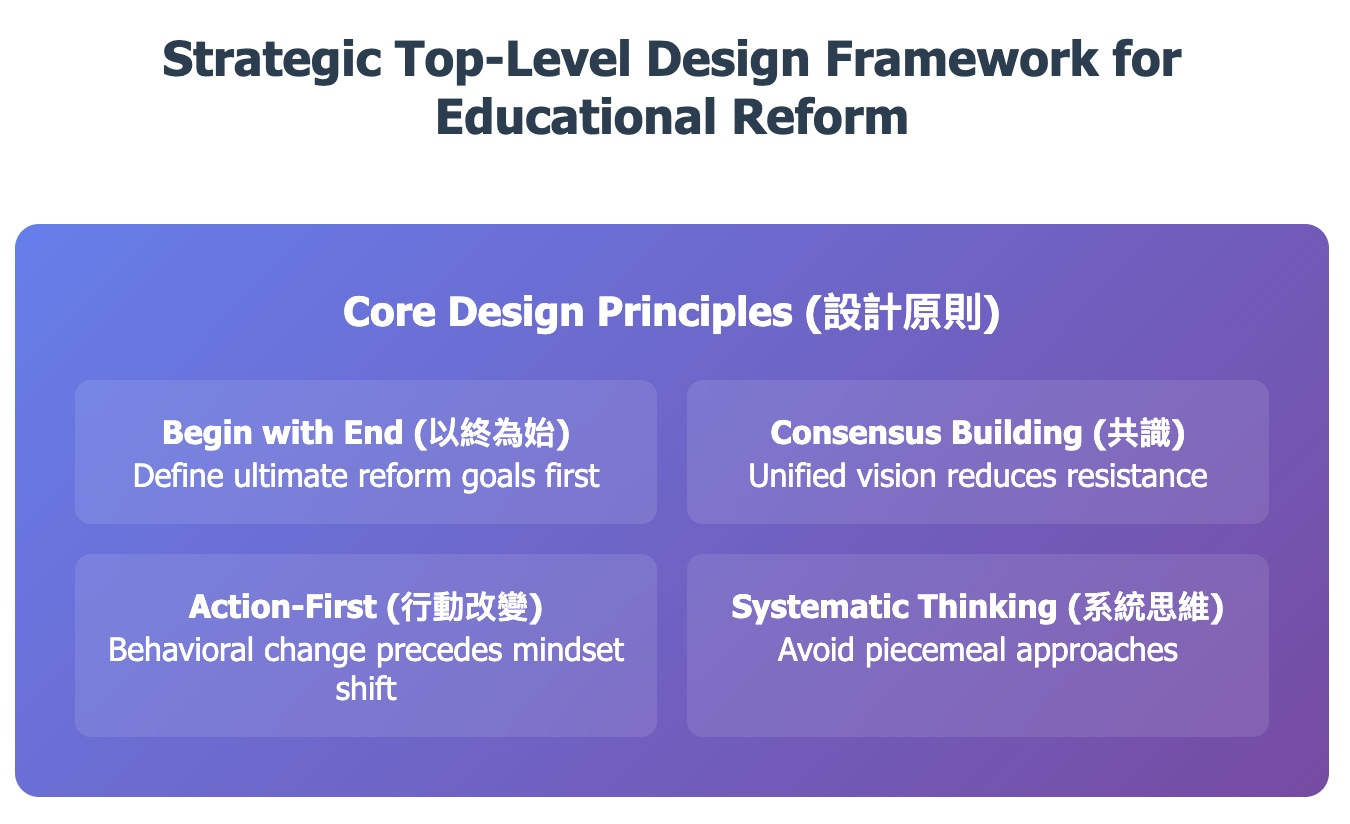
\includegraphics[keepaspectratio]{_resources/images/Ch3-Strategy.jpg}}

\section{Systems Thinking in Educational
Design}\label{systems-thinking-in-educational-design}

Strategic top-level design demands sophisticated systems thinking that
recognizes the complex interdependencies within educational
environments. Unlike mechanical systems where components function
independently, educational systems exhibit what complexity theorists
call ``emergent properties'' --- outcomes that arise from the
interaction of multiple elements rather than from any single
intervention.

Systems thinking in educational design requires leaders to map the
relationships between seemingly separate elements. Teacher beliefs about
learning influence classroom practices, which shape student
expectations, which affect learning outcomes, which inform parent
perceptions, which influence policy decisions, which determine resource
allocation, which affects teacher working conditions, completing the
cycle. Effective strategic design identifies these feedback loops and
designs interventions that create positive rather than negative
reinforcement patterns.

The inquiry-based learning transformation exemplifies systems thinking
in practice. Successful implementation requires alignment across
multiple system levels: individual teacher beliefs and practices,
departmental collaboration patterns, administrative support structures,
assessment and evaluation systems, parent and community expectations,
and broader policy frameworks. Misalignment at any level can undermine
the entire transformation effort.

Regional experiences from Jilin Province illustrate this systems
approach. Rather than simply training teachers in inquiry methods,
educational leaders simultaneously redesigned evaluation systems to
reward student questioning rather than just correct answers,
restructured professional development to emphasize collaborative
investigation rather than individual skill acquisition, and engaged
parents in understanding how inquiry learning would benefit their
children's long-term development. This multi-level coordination created
reinforcing pressures that supported rather than undermined the desired
transformation.

Systems thinking also reveals the importance of what change theorists
call ``leverage points'' --- places within complex systems where small
shifts can produce significant changes. In educational transformation,
these leverage points often exist at the intersection of formal and
informal structures. For example, changing how teachers collaborate
informally can have greater impact than modifying official curriculum
documents, because informal collaboration patterns influence how
teachers interpret and implement formal requirements.

\section{The Backwards Design
Methodology}\label{the-backwards-design-methodology}

Backwards design methodology provides the operational framework for
translating strategic vision into practical implementation plans. This
approach, pioneered in curriculum development by Grant Wiggins and Jay
McTighe, proves particularly powerful in comprehensive educational
transformation because it maintains focus on ultimate outcomes while
allowing flexibility in implementation pathways.

The methodology operates through three sequential stages, each building
upon the previous one. First, leaders identify desired results with
specific, measurable outcomes that define successful transformation.
Second, they determine acceptable evidence that would demonstrate
achievement of those outcomes. Third, they design learning experiences
and instruction that will produce the acceptable evidence and achieve
the desired results.

Applied to inquiry-based learning transformation, backwards design
begins with precise specification of inquiry capabilities that graduates
should demonstrate. These might include the ability to generate
researchable questions from complex scenarios, design and conduct
systematic investigations using appropriate methodologies, analyze
evidence critically to draw warranted conclusions, and communicate
findings effectively to diverse audiences. Each capability must be
defined with sufficient clarity that progress can be measured and
supported.

The evidence determination stage requires leaders to specify how they
will recognize successful development of inquiry capabilities. This
stage proves particularly challenging in inquiry-based systems because
traditional assessment methods often conflict with inquiry principles.
If leaders want students to develop questioning abilities, they must
create assessment systems that reward good questions rather than just
correct answers. If they want students to pursue independent
investigations, they must develop evaluation methods that assess
investigative processes rather than just final products.

Dongfeng County's experience illustrates effective backwards design
implementation. County leaders began by specifying that successful
students would demonstrate curiosity-driven questioning, evidence-based
reasoning, and collaborative problem-solving. They then identified
evidence including student-generated research questions, investigation
portfolios, peer evaluation of collaborative work, and parent reports of
increased questioning at home. Finally, they designed professional
development, curriculum modifications, and classroom practice changes
that would produce this evidence.

The learning experience design stage requires careful attention to the
developmental sequence through which inquiry capabilities emerge. Unlike
content knowledge that can be transmitted directly, inquiry capabilities
develop through guided practice with gradually increasing independence.
This development requires teachers to shift from information delivery
toward what the Chinese reform documents call ``导练'' (dǎo liàn) ---
guided practice that scaffolds student exploration while maintaining
clear learning objectives.

\section{Implementation Frameworks}\label{implementation-frameworks}

Strategic implementation requires frameworks that maintain coherence
while allowing adaptation to local contexts. The most effective
frameworks provide sufficient structure to ensure consistency while
preserving flexibility needed for contextual responsiveness. This
balance proves particularly important in inquiry-based learning
implementation because questioning and exploration must be authentic to
students' lived experiences while building toward systematic
investigation capabilities.

Successful implementation frameworks typically include four essential
components: phase sequencing, stakeholder engagement protocols,
monitoring and adjustment mechanisms, and sustainability planning. Each
component must be designed to support inquiry-based learning principles
while addressing practical implementation challenges.

Phase sequencing involves careful planning of transformation stages that
build capability incrementally while maintaining institutional
stability. The Chinese reform experiences suggest that effective
sequencing begins with pilot implementations in supportive environments,
expands to broader implementation as capabilities develop, and finally
integrates inquiry approaches throughout entire systems. This sequencing
allows for learning and adjustment while building confidence and
competence among stakeholders.

The pilot phase serves multiple purposes beyond simply testing new
approaches. Pilots create local expertise that can support broader
implementation, generate concrete examples that help other educators
understand inquiry-based practices, and provide evidence of
effectiveness that builds stakeholder confidence. However, pilots must
be designed as learning laboratories rather than demonstration projects,
with explicit mechanisms for capturing lessons and adapting approaches
based on experience.

Stakeholder engagement protocols ensure that all affected parties
understand their roles in supporting inquiry-based learning
transformation. These protocols must address parents who may worry that
questioning-focused education will undermine academic achievement,
teachers who may feel unprepared to facilitate rather than direct
student learning, and administrators who may need to restructure
evaluation and support systems. Effective engagement moves beyond simple
communication toward active involvement in transformation planning and
implementation.

Monitoring and adjustment mechanisms provide the feedback systems
necessary for adaptive implementation. Traditional project management
approaches often prove inadequate for educational transformation because
learning systems exhibit nonlinear responses to interventions. Small
changes can sometimes produce dramatic results, while major
interventions may have minimal impact. Effective monitoring systems
track both intended and unintended consequences while providing
mechanisms for rapid adjustment when implementation deviates from
desired directions.

\section{Avoiding Design Pitfalls}\label{avoiding-design-pitfalls}

Strategic design efforts face several common pitfalls that can undermine
even well-intentioned transformation efforts. Recognizing and avoiding
these pitfalls proves essential for successful inquiry-based learning
implementation. The Chinese reform documents specifically warn against
``形式主义'' (xíngshì zhǔyì) --- formalism that focuses on surface
appearances rather than substantive change --- and ``拿来主义'' (ná lái
zhǔyì) --- borrowing approaches without adaptation to local contexts.

Formalism represents perhaps the most insidious design pitfall because
it creates the appearance of transformation without achieving
substantive change. In inquiry-based learning contexts, formalism might
involve teachers asking more questions during lessons without actually
shifting toward student-generated inquiry, or schools adopting inquiry
terminology while maintaining traditional evaluation systems that reward
compliance rather than questioning. Avoiding formalism requires leaders
to focus on outcomes rather than activities, measuring actual changes in
student questioning and investigation capabilities rather than simply
counting inquiry-based lesson plans.

The borrowing pitfall occurs when leaders attempt to import successful
practices from other contexts without adequate attention to local
conditions. While learning from successful examples proves valuable,
direct replication rarely succeeds because educational practices emerge
from complex interactions between formal structures, informal culture,
resource availability, and stakeholder expectations. Effective strategic
design adapts promising practices to local contexts rather than
importing them wholesale.

A third major pitfall involves what we might call ``implementation
compression'' --- attempting to accelerate transformation beyond the
natural pace of capability development. Educational transformation
requires time for stakeholders to develop new knowledge, skills, and
attitudes. Rushing implementation often produces surface compliance
without deep understanding, creating fragile changes that disappear when
external pressure diminishes. Strategic design must account for the time
required for authentic transformation while maintaining momentum and
stakeholder engagement.

Scope creep represents another common pitfall where strategic design
efforts expand beyond manageable boundaries. While comprehensive
transformation requires attention to multiple system elements,
attempting to change everything simultaneously can overwhelm
stakeholders and fragment leadership attention. Effective strategic
design prioritizes high-leverage interventions while sequencing
additional changes to build on initial successes.

\section{Integration with Organizational
Culture}\label{integration-with-organizational-culture}

Strategic top-level design must account for the deep cultural patterns
that shape how educational organizations function. Culture influences
everything from how teachers collaborate to how students perceive their
roles as learners. Inquiry-based learning transformation requires
cultural shifts that support questioning, exploration, and intellectual
risk-taking --- qualities that may conflict with traditional educational
cultures emphasizing compliance, standardization, and certainty.

Cultural integration begins with understanding existing cultural
patterns and their relationship to inquiry-based learning goals.
Traditional educational cultures often reward students for producing
correct answers quickly rather than asking thoughtful questions,
teachers for maintaining classroom control rather than facilitating
student exploration, and administrators for achieving predictable
outcomes rather than supporting innovative practices. These cultural
patterns create what organizational theorists call ``institutional
friction'' that can undermine even well-designed transformation efforts.

Effective cultural integration requires what Edgar Schein calls
``cultural learning'' --- processes through which organizations develop
new shared assumptions about effective practice. This learning cannot be
mandated through policy changes but must emerge through sustained
experience with new approaches that demonstrate superior outcomes.
Strategic design must create opportunities for stakeholders to
experience the benefits of inquiry-based learning directly rather than
simply hearing about them abstractly.

The Chinese reform experiences demonstrate several effective cultural
integration strategies. School leaders created ``learning communities''
where teachers collaborated in developing and refining inquiry-based
practices, providing social support for cultural change. They celebrated
examples of effective student questioning and investigation, gradually
shifting recognition systems toward inquiry-based achievements. They
engaged parents in understanding how inquiry learning would benefit
their children, building community support for cultural transformation.

Cultural integration also requires attention to what anthropologists
call ``cultural artifacts'' --- the visible symbols, stories, and
practices that embody organizational values. In inquiry-based learning
transformation, these artifacts might include classroom arrangements
that support collaborative investigation, display systems that showcase
student questions alongside their answers, and evaluation forms that
assess questioning capabilities alongside content knowledge.

\section{Conclusion}\label{conclusion}

Strategic top-level design provides the foundation upon which successful
educational transformation builds. By beginning with clear vision,
thinking systemically about complex interdependencies, employing
backwards design methodology, implementing through structured
frameworks, avoiding common pitfalls, and integrating with
organizational culture, educational leaders can create coherent
transformation processes that achieve sustainable change.

The inquiry-based learning transformation demands particularly
sophisticated strategic design because it requires alignment across
multiple system levels while supporting the development of complex
capabilities that emerge through guided practice rather than direct
instruction. Success requires leaders who can think architecturally
about educational systems while remaining responsive to local contexts
and stakeholder needs.

As we will explore in subsequent chapters, strategic design provides the
framework within which specific implementation strategies, leadership
approaches, and teacher development programs can be organized and
coordinated. Without this strategic foundation, even excellent specific
practices may fail to achieve their potential impact because they lack
the systemic support necessary for sustainable transformation.

The Chinese reform experiences demonstrate that strategic top-level
design, when implemented thoughtfully and persistently, can create
educational environments where students develop as confident, capable
inquirers prepared to address the complex challenges of an uncertain
future. This achievement requires leaders who understand that
transformation is not about changing what schools do, but about changing
what schools are --- their fundamental identity, purpose, and way of
being in the world.

\bookmarksetup{startatroot}

\chapter{The Three Questions, Three Explorations
Model}\label{the-three-questions-three-explorations-model}

\section{Introduction}\label{introduction-2}

The Three Questions, Three Explorations (三疑三探: sān yí sān tàn)
pedagogical framework represents a systematic approach to inquiry-based
learning that fundamentally reconceptualizes the relationship between
teacher, student, and knowledge. Rather than positioning educators as
knowledge transmitters and students as passive recipients, this model
creates dynamic learning environments where questioning becomes the
primary vehicle for intellectual development and understanding emerges
through structured exploration.

This methodology emerged from extensive educational research and
practical implementation across diverse institutional contexts,
demonstrating remarkable adaptability while maintaining core pedagogical
principles. The framework's strength lies not in its rigid application
but in its capacity to be contextualized within specific educational
environments while preserving the essential elements that drive student
engagement and deep learning.

\section{Theoretical Foundations}\label{theoretical-foundations}

The Three Questions, Three Explorations model rests on several
interconnected theoretical premises that challenge conventional
educational assumptions. The foundational principle centers on epistemic
trust in students---the belief that learners possess inherent capacity
for critical thinking and knowledge construction when provided with
appropriate scaffolding and opportunities for intellectual exploration.

This epistemic framework draws from constructivist learning theory,
which posits that knowledge is actively constructed rather than
passively received. Students bring prior experiences, cultural
knowledge, and intuitive understanding to learning situations, and
effective pedagogy leverages these existing cognitive resources as
building blocks for new understanding. The model recognizes that
authentic learning occurs when students grapple with genuine questions
and problems that connect to their lived experiences and intellectual
curiosity.

The questioning component of the framework aligns with Socratic
pedagogical traditions while incorporating contemporary understanding of
metacognitive development. By teaching students to formulate meaningful
questions, educators develop learners' capacity for self-directed
inquiry and critical evaluation of information sources. This questioning
competence becomes a transferable skill that extends beyond specific
subject matter into lifelong learning capabilities.

\section{The Three Questions
Framework}\label{the-three-questions-framework}

The questioning dimension of the model operates through three distinct
but interconnected phases that progressively deepen student engagement
with content and concepts. Each phase serves specific pedagogical
functions while contributing to the overall development of critical
thinking capabilities.

\subsection{Initial Questioning Phase}\label{initial-questioning-phase}

The first questioning phase focuses on activating prior knowledge and
establishing conceptual connections between new content and existing
understanding. Students are encouraged to generate questions that emerge
from their initial encounter with material, whether through reading
assignments, multimedia presentations, or hands-on experiences. These
questions typically reflect curiosity about surface-level features or
apparent contradictions between new information and previously held
beliefs.

Effective facilitation during this phase requires educators to model
questioning strategies while avoiding the temptation to provide
immediate answers. Instead, teachers guide students toward recognizing
the types of questions that promote deeper investigation and
understanding. This phase serves as intellectual preparation for more
sophisticated inquiry by establishing a foundation of student-generated
questions that will drive subsequent exploration.

The initial questioning phase also functions as a diagnostic tool,
revealing student preconceptions, areas of confusion, and existing
knowledge gaps. This information proves invaluable for educators in
tailoring subsequent learning experiences to address specific student
needs and interests while building upon demonstrated strengths and
understanding.

\subsection{Analytical Questioning
Phase}\label{analytical-questioning-phase}

The second questioning phase shifts focus toward analytical and
evaluative inquiry that examines relationships between concepts,
identifies underlying patterns, and explores implications of new
understanding. Students develop skills in formulating questions that
probe beneath surface appearances to examine causal relationships,
structural similarities, and conceptual frameworks.

During this phase, students learn to distinguish between questions that
seek factual information and those that promote analytical thinking.
They develop facility with question stems that encourage comparison,
evaluation, synthesis, and application of concepts across different
contexts. This questioning sophistication reflects growing metacognitive
awareness as students become more conscious of their own thinking
processes and learning strategies.

The analytical questioning phase often involves collaborative inquiry
where students build upon each other's questions and perspectives. This
social dimension of questioning helps students recognize the value of
diverse viewpoints and the collective nature of knowledge construction.
Students learn to refine their questions through peer interaction and
develop appreciation for the iterative nature of inquiry.

\subsection{Synthetic Questioning
Phase}\label{synthetic-questioning-phase}

The final questioning phase emphasizes synthetic thinking that connects
learning across disciplinary boundaries and explores implications for
real-world applications. Students formulate questions that examine how
new understanding relates to broader social, ethical, or practical
concerns. This phase develops capacity for transfer of learning and
application of academic knowledge to authentic problem-solving
situations.

Synthetic questioning requires students to move beyond content mastery
toward consideration of knowledge's significance and utility. Students
explore questions such as how new understanding changes their
perspective on related issues, what actions or decisions might be
informed by this knowledge, and how concepts might apply in different
contexts or circumstances.

This phase often involves students in generating questions for future
investigation, developing research proposals, or identifying areas where
additional learning is needed. The synthetic questioning phase thus
connects current learning to ongoing intellectual development and
establishes foundations for self-directed learning beyond formal
educational settings.

\section{The Three Explorations
Framework}\label{the-three-explorations-framework}

The exploration component of the model provides structured opportunities
for students to investigate their questions through diverse learning
modalities and investigation strategies. Each exploration phase
corresponds to different levels of cognitive engagement and
progressively develops students' capacity for independent inquiry and
knowledge construction.

\subsection{Guided Exploration}\label{guided-exploration}

The first exploration phase provides structured investigation
opportunities where students explore questions within carefully designed
learning environments. Teachers establish parameters for investigation
while allowing sufficient flexibility for student agency and discovery.
This phase might involve laboratory experiments, document analysis,
field observations, or collaborative problem-solving activities that
address student-generated questions.

Guided exploration serves multiple pedagogical functions simultaneously.
It develops students' investigative skills while ensuring that
exploration remains focused and productive. Teachers provide scaffolding
that helps students navigate complex information sources, apply
appropriate analytical tools, and maintain systematic approaches to
inquiry. This support prevents the frustration that can occur when
students lack sufficient background knowledge or methodological
understanding to pursue independent investigation effectively.

The guided exploration phase also establishes communities of inquiry
where students learn from peer interaction and collaborative
investigation. Students discover that multiple investigation strategies
can address similar questions and that diverse perspectives enhance
understanding. This collaborative dimension helps students develop
communication skills and appreciation for the social nature of knowledge
construction.

\subsection{Independent Exploration}\label{independent-exploration}

The second exploration phase transitions responsibility for
investigation design and implementation to students while maintaining
teacher availability for consultation and guidance. Students select
investigation methods, identify relevant resources, and develop
systematic approaches to addressing their questions. This phase develops
autonomy and self-direction while building confidence in students'
capacity for independent learning.

Independent exploration requires students to apply metacognitive
strategies as they monitor their own learning progress and adjust
investigation approaches based on emerging findings. Students develop
skills in time management, resource evaluation, and systematic
documentation of investigation processes and outcomes. These
transferable skills prove valuable across academic disciplines and in
professional contexts.

The independent exploration phase often reveals individual student
interests and strengths while providing opportunities for differentiated
learning experiences. Students pursue investigations that align with
their curiosity and learning preferences while developing expertise in
self-directed inquiry. Teachers serve as consultants who provide
feedback and suggestions while respecting student ownership of the
investigation process.

\subsection{Collaborative Exploration}\label{collaborative-exploration}

The final exploration phase involves students in collective
investigation projects that address complex questions requiring diverse
expertise and perspectives. Students form investigation teams based on
shared interests or complementary skills and work together to design and
implement comprehensive inquiry projects. This phase develops
collaboration skills while tackling sophisticated questions that exceed
individual student capacity.

Collaborative exploration introduces students to the distributed nature
of expertise and the importance of interdisciplinary approaches to
complex problems. Students learn to negotiate different viewpoints,
integrate diverse investigation methods, and synthesize findings from
multiple sources. These collaborative skills prepare students for
professional environments where teamwork and collective problem-solving
are essential capabilities.

The collaborative exploration phase often involves students in authentic
research projects that contribute to broader knowledge communities.
Students might conduct original research, develop solutions to community
problems, or create resources that benefit other learners. This
authentic dimension enhances student motivation while demonstrating the
real-world relevance of academic inquiry skills.

\section{Implementation Strategies}\label{implementation-strategies}

Successful implementation of the Three Questions, Three Explorations
model requires careful attention to classroom culture, assessment
practices, and teacher preparation. The model represents a significant
departure from traditional instructional approaches and requires
sustained support for both educators and students as they adapt to new
roles and expectations.

\subsection{Classroom Environment
Design}\label{classroom-environment-design}

Creating environments that support inquiry-based learning involves both
physical and cultural considerations. Classrooms must provide
flexibility for diverse learning configurations, from individual
reflection to small group collaboration to large group discussion.
Technology integration should support investigation and communication
rather than replacing human interaction and critical thinking.

The cultural dimension of classroom environment proves equally
important. Students must feel safe to ask questions, propose hypotheses,
and share tentative understanding without fear of judgment or ridicule.
Teachers establish norms that value intellectual risk-taking, celebrate
productive mistakes, and recognize diverse forms of contribution to
collective learning.

Assessment practices must align with inquiry-based learning objectives
by evaluating process as well as product and recognizing growth over
time rather than focusing exclusively on final outcomes. Formative
assessment strategies help students monitor their own learning progress
while providing teachers with information needed to adjust instruction
and support.

\subsection{Teacher Professional
Development}\label{teacher-professional-development}

Implementing the Three Questions, Three Explorations model requires
significant investment in teacher professional development that
addresses both pedagogical skills and mindset shifts. Teachers must
develop facility with questioning strategies, investigation design, and
collaborative learning facilitation while examining their own beliefs
about knowledge, learning, and student capability.

Professional development should include opportunities for teachers to
experience inquiry-based learning as participants before attempting to
facilitate such experiences for their students. This experiential
learning helps educators understand the cognitive and emotional
dimensions of inquiry while building confidence in their ability to
navigate the uncertainty that characterizes authentic learning
environments.

Ongoing support structures prove essential for sustaining implementation
efforts. Teachers benefit from professional learning communities where
they can share experiences, problem-solve challenges, and reflect on
their practice with colleagues who are engaged in similar transformation
efforts. Administrators must provide time, resources, and encouragement
for this collaborative professional development.

\section{Innovation Points and
Adaptations}\label{innovation-points-and-adaptations}

The Three Questions, Three Explorations model incorporates several
innovative features that distinguish it from other inquiry-based
approaches while maintaining flexibility for local adaptation. These
innovation points reflect lessons learned from extensive implementation
experience across diverse educational contexts.

The integration of self-compiled practice materials allows students to
create their own learning resources based on their investigation
findings. This approach develops synthesis skills while ensuring that
learning materials remain current and relevant to student interests.
Students become content creators rather than passive consumers of
pre-packaged educational materials.

Systematic questioning and follow-up procedures ensure that inquiry
remains focused and productive rather than wandering without direction.
Students learn to pursue questions with persistence while recognizing
when investigation approaches need modification or when additional
expertise is required. This balance between intellectual curiosity and
systematic investigation develops both creativity and rigor.

End-of-class assessment practices provide regular opportunities for
students to demonstrate understanding while identifying areas requiring
additional investigation. These assessments serve formative functions by
informing subsequent learning activities rather than simply evaluating
student performance. The assessment process becomes part of the learning
cycle rather than an external judgment of learning outcomes.

\section{Conclusion}\label{conclusion-1}

The Three Questions, Three Explorations model represents a comprehensive
approach to inquiry-based education that addresses both cognitive and
affective dimensions of learning. By systematically developing students'
questioning abilities and providing structured opportunities for
investigation, the model creates learning environments where
intellectual curiosity drives educational engagement and deep
understanding emerges through active construction of knowledge.

Successful implementation requires sustained commitment from educational
leaders, comprehensive teacher preparation, and supportive institutional
structures as discussed in Chapters 2, 5, and 6. The model's flexibility
allows for adaptation to diverse contexts while maintaining core
principles that promote student agency, critical thinking, and
collaborative learning.

The framework's emphasis on questioning and exploration prepares
students for lifelong learning in rapidly changing social and
technological environments. As traditional approaches to education prove
increasingly inadequate for preparing students for uncertain futures,
the Three Questions, Three Explorations model offers a robust
alternative that develops transferable thinking skills and intellectual
dispositions essential for navigating complexity and ambiguity. The
model thus serves not merely as an instructional strategy but as
preparation for engaged citizenship and professional effectiveness in
democratic societies that require citizens capable of critical thinking
and collaborative problem-solving.

\bookmarksetup{startatroot}

\chapter{Leadership in Educational
Innovation}\label{leadership-in-educational-innovation}

\section{Introduction}\label{introduction-3}

Educational transformation requires more than good intentions and sound
pedagogical theory. At its core, sustainable reform depends on leaders
who possess both the vision to imagine radically different educational
futures and the practical wisdom to navigate the complex human dynamics
inherent in institutional change. This chapter examines the multifaceted
role of leadership in driving inquiry-based educational reform,
exploring how administrators, principals, and teacher leaders can
effectively guide their institutions through the challenging but
essential process of transformation.

The Chinese concept of \emph{zhǐhuī} (指挥), meaning to command or
direct, captures only part of what educational leadership requires
during reform initiatives. More apt is the notion of \emph{yǐndǎo}
(引导), which suggests guidance that draws others forward rather than
pushing from behind. Effective educational leaders must master this
subtle distinction, understanding when to provide clear direction and
when to create conditions for organic growth and development.

\section{The Paradox of Educational
Leadership}\label{the-paradox-of-educational-leadership}

Educational leaders face a fundamental paradox during reform
initiatives. They must simultaneously demonstrate unwavering commitment
to change while remaining flexible enough to adapt their approaches
based on emerging evidence and evolving circumstances. This tension
between conviction and adaptability often determines whether reform
efforts succeed or fail.

Consider the experience of principals who have successfully implemented
inquiry-based learning models. They typically begin with what Heidegger
might call a \emph{Vorlauf} (running ahead) - a projective understanding
of where their institution needs to go. Yet they must also maintain what
he termed \emph{Gelassenheit} (letting-be), an openness to how that
transformation might unfold in ways they cannot fully anticipate or
control.

This paradox manifests in several key areas. Leaders must articulate
compelling visions while acknowledging uncertainty about specific
outcomes. They must make decisive resource allocation decisions while
remaining open to course corrections. Perhaps most challenging, they
must project confidence in their strategic direction while modeling the
intellectual humility that inquiry-based learning itself demands.

\section{Breaking Out of Institutional Comfort
Zones}\label{breaking-out-of-institutional-comfort-zones}

One of the most critical functions of educational leadership during
reform is disrupting established patterns of practice and thinking.
Schools, like all institutions, develop what organizational theorists
call ``dynamic conservatism'' - a tendency to maintain existing
structures and processes even when they no longer serve their intended
purposes effectively.

The comfort zone phenomenon in educational settings operates at multiple
levels. Individual teachers may resist new pedagogical approaches that
challenge their established expertise. Departments may protect
curriculum territories that reflect historical power distributions
rather than current student needs. Parent communities may advocate for
familiar practices that mirror their own educational experiences,
regardless of their current relevance or effectiveness.

Effective reform leaders understand that breaking out of these comfort
zones requires both strategic thinking and emotional intelligence.
Simply mandating change often produces compliance without commitment,
resulting in superficial implementation that lacks the depth necessary
for genuine transformation. Instead, successful leaders create what we
might call ``productive discomfort'' - conditions that challenge
existing assumptions while providing sufficient support and resources to
enable meaningful adaptation.

This process often begins with what the documents describe as ``thinking
leadership'' (\emph{sīgēn yǐnlǐng} 思根引领). Leaders must first
articulate why current practices fall short of educational ideals and
how inquiry-based approaches offer more promising alternatives. This
requires both analytical rigor in diagnosing current challenges and
imaginative capacity in envisioning better possibilities.

\section{Establishing Models and Creating
Momentum}\label{establishing-models-and-creating-momentum}

Once leaders have successfully disrupted existing comfort zones, they
face the challenge of providing concrete alternatives that teachers and
students can understand and implement. This is where the strategy of
``establishing models'' (\emph{shùlì biāogǎn} 树立标杆) becomes crucial.

The most effective educational leaders recognize that teachers need
tangible examples of successful practice, not just theoretical
frameworks. They identify early adopters within their institutions -
often informal teacher leaders who possess both pedagogical skill and
collegial credibility - and provide them with additional support and
resources to develop exemplary implementations of inquiry-based
approaches.

These model classrooms serve multiple functions. They demonstrate that
inquiry-based learning is practically feasible within existing
constraints of time, resources, and accountability requirements. They
provide venues for collaborative observation and reflection, allowing
skeptical colleagues to see new approaches in action rather than simply
hearing about them in abstract terms. Perhaps most importantly, they
create positive peer pressure by making innovative practice visible and
celebrated within the school community.

The process of establishing models requires careful attention to
selection criteria and support mechanisms. Leaders must identify
teachers who possess not only strong instructional skills but also the
interpersonal abilities necessary to mentor colleagues and the
reflective capacity to articulate their practice clearly. They must
provide these model teachers with adequate preparation time, appropriate
resources, and ongoing coaching to ensure their success.

Successful model development also requires what we might call
``intelligent scaffolding.'' Rather than expecting teachers to implement
completely new approaches overnight, effective leaders break down
complex reforms into manageable components that can be learned and
integrated gradually. This might involve focusing initially on
questioning techniques, then adding collaborative learning structures,
and finally incorporating assessment approaches that align with
inquiry-based principles.

\section{Institutional Promotion and Systemic
Support}\label{institutional-promotion-and-systemic-support}

Creating individual models of excellence represents an important first
step, but sustainable reform requires broader institutional changes that
support and reinforce new practices. This is where the strategy of
``institutional promotion'' (\emph{zhìdù tuīdòng} 制度推动) becomes
essential.

Educational leaders must recognize that individual teacher behavior is
profoundly shaped by institutional context. Grading policies, scheduling
structures, professional development offerings, evaluation criteria, and
resource allocation patterns all send powerful messages about what the
organization actually values, regardless of what mission statements or
strategic plans might claim.

Effective reform leaders undertake systematic reviews of these
institutional policies and practices, identifying misalignments between
stated commitments to inquiry-based learning and existing organizational
structures. They then work deliberately to modify policies and create
new structures that support rather than undermine innovative practice.

This work often requires considerable political skill, as institutional
policies typically reflect complex negotiations among various
stakeholder groups with different priorities and interests. Leaders must
build coalitions of support for policy changes while managing resistance
from groups that benefit from existing arrangements. They must also
sequence policy modifications carefully, ensuring that new requirements
do not overwhelm teachers who are already managing significant
pedagogical changes.

One particularly important aspect of institutional promotion involves
developing new evaluation and assessment systems that align with
inquiry-based learning principles. Traditional accountability measures
often emphasize standardized test scores and other quantitative metrics
that may not capture the full range of learning outcomes that
inquiry-based approaches seek to promote. Leaders must work with their
communities to develop more comprehensive assessment approaches that
include measures of critical thinking, collaborative problem-solving,
and student engagement alongside traditional academic indicators.

\section{The Strategic Dimensions of Educational
Leadership}\label{the-strategic-dimensions-of-educational-leadership}

Effective educational leaders during reform periods must think
strategically about both immediate implementation challenges and
longer-term sustainability requirements. This involves what military
strategists call ``operating on multiple time horizons'' - managing
current tactical decisions while maintaining awareness of broader
strategic objectives.

The documents emphasize the importance of leaders having both
\emph{zhànlüè} (战略, strategy) and firm conviction (\emph{jiāndìng de
xìnniàn hé juéxīn} 坚定的信念和决心). This combination proves essential
because educational reform typically requires sustained effort over
multiple years before significant results become visible. Leaders must
maintain institutional momentum through inevitable periods of difficulty
and uncertainty.

Strategic thinking in educational reform involves several key
components. Leaders must develop realistic timelines that account for
the iterative nature of pedagogical change. They must anticipate likely
sources of resistance and develop proactive responses. They must
identify critical resource needs and secure sustainable funding streams.
Perhaps most importantly, they must build organizational capacity for
continuous learning and adaptation.

This last point deserves particular emphasis. The most successful
educational leaders understand that inquiry-based learning represents
not just a new teaching methodology but a fundamentally different
approach to organizational learning. They model the same questioning,
exploring, and reflecting behaviors that they ask teachers to
demonstrate in their classrooms. They create structures for systematic
data collection and analysis about reform implementation. They encourage
experimentation and treat failures as learning opportunities rather than
sources of blame or punishment.

\section{Avoiding Common Leadership
Pitfalls}\label{avoiding-common-leadership-pitfalls}

The documents warn against several dangerous tendencies that can
undermine educational reform efforts: formalism (\emph{xíngshìzhǔyì}
形式主义), blind adoption (\emph{nálái zhǔyì} 拿来主义), and rushed
implementation (\emph{mángmù yuèjìn} 盲目跃进). Educational leaders must
understand how these pitfalls manifest and develop strategies for
avoiding them.

Formalism occurs when leaders focus more on the appearance of reform
than its substance. This might involve mandating specific lesson plan
formats without ensuring that teachers understand the pedagogical
principles underlying those formats. Or it might involve implementing
inquiry-based learning ``models'' without providing teachers with
adequate time and support to develop the complex facilitation skills
these approaches require.

Blind adoption represents another common pitfall. Leaders may observe
successful practices in other contexts and attempt to transplant them
directly into their own institutions without adequate attention to local
conditions and constraints. While learning from external examples proves
valuable, effective leaders understand that successful practices must be
adapted rather than simply copied.

Rushed implementation creates perhaps the most dangerous pitfall of all.
Facing pressure from superintendents, school boards, or community
members for rapid improvements, leaders may attempt to implement
comprehensive reforms too quickly. This typically overwhelms teachers
and produces superficial compliance rather than genuine transformation.
The documents emphasize that ``new models mature and standardize through
repeated application, continuous exploration, and research'' - a process
that requires patience and persistence from educational leaders.

\section{Building Organizational Learning
Capacity}\label{building-organizational-learning-capacity}

Perhaps the most important long-term contribution that educational
leaders can make involves building their institutions' capacity for
continuous learning and improvement. This requires moving beyond
episodic reform initiatives toward what organizational theorists call
``learning organizations'' - institutions that systematically gather
information about their performance, reflect on that information
thoughtfully, and modify their practices based on what they learn.

Creating learning organizations in educational contexts requires
attention to both structural and cultural dimensions. Structurally,
leaders must establish regular opportunities for collaborative
reflection and professional dialogue. This might involve implementing
lesson study protocols, creating teacher inquiry groups, or establishing
data analysis teams. The specific mechanisms matter less than ensuring
that such opportunities exist consistently and are well-supported.

Culturally, leaders must work to establish norms that encourage
intellectual risk-taking and honest self-assessment. Teachers must feel
safe to admit uncertainty, request help, and experiment with new
approaches without fear of negative evaluation. This requires leaders to
model such behaviors themselves and to celebrate learning from failure
as much as they celebrate conventional success.

The development of organizational learning capacity also requires
attention to what Chris Argyris called ``double-loop learning'' - the
ability to question not just specific practices but the underlying
assumptions and beliefs that guide those practices. In educational
contexts, this means encouraging teachers and administrators to examine
their fundamental beliefs about student capabilities, effective
pedagogy, and the purposes of education itself.

\section{Conclusion}\label{conclusion-2}

Leadership in educational innovation requires a sophisticated
understanding of both technical and adaptive challenges. Technical
challenges involve implementing known solutions to well-defined problems
- establishing new curriculum materials, training teachers in specific
instructional strategies, or modifying assessment procedures. Adaptive
challenges involve changing hearts and minds, shifting organizational
cultures, and developing new capabilities in response to complex and
evolving circumstances.

The most effective educational leaders recognize that inquiry-based
learning reform presents primarily adaptive challenges that cannot be
solved through technical solutions alone. They understand that
sustainable change requires patient, persistent work to shift mindsets,
build capabilities, and create supportive organizational conditions.
They approach this work with both strategic clarity about desired
outcomes and tactical flexibility about implementation pathways.

As we will explore in subsequent chapters, the leadership strategies
discussed here must be complemented by careful attention to teacher
development (Chapter 7), systematic approaches to scaling successful
practices (Chapter 6), and robust evaluation systems that can provide
feedback for continuous improvement (Chapter 9). Educational
transformation represents a complex, multifaceted endeavor that requires
sustained leadership commitment and sophisticated strategic thinking,
but the potential rewards - for students, teachers, and communities -
justify the considerable effort required.

\bookmarksetup{startatroot}

\chapter{From Pilot Programs to System-Wide
Implementation}\label{from-pilot-programs-to-system-wide-implementation}

\section{Introduction}\label{introduction-4}

The transition from isolated pilot programs to comprehensive system-wide
implementation represents one of the most critical phases in educational
transformation. While pilot programs serve as essential proof-of-concept
vehicles for testing innovative approaches like inquiry-based learning,
their ultimate value lies in their ability to scale successfully across
entire educational systems. This chapter examines the systematic
progression from experimental initiatives to institutional change,
drawing on case studies and implementation frameworks that have
demonstrated sustainable success in transforming educational practices.

The scaling challenge fundamentally differs from pilot program
management. Where pilots typically operate with carefully selected
participants, additional resources, and intensive oversight, system-wide
implementation must function within existing constraints while
maintaining the pedagogical integrity that made the pilot successful.
This transition requires sophisticated understanding of organizational
change dynamics, stakeholder management, and the cultural transformation
processes discussed in Chapter 2 on building consensus and shared
vision.

\section{The Scaling Imperative}\label{the-scaling-imperative}

Educational systems worldwide face mounting pressure to move beyond
incremental improvements toward transformational change. Traditional
approaches to educational innovation often remain trapped in what
researchers term the ``pilot purgatory'' --- endless cycles of
small-scale experiments that never achieve the scale necessary for
meaningful impact. The urgency of this challenge has intensified as
digital transformation and changing workforce demands require
fundamentally different educational outcomes.

The inquiry-based learning approaches exemplified by the Three
Questions, Three Explorations model (三疑三探) demonstrate particular
promise for scaling because they align with universal principles of
cognitive development while remaining adaptable to diverse cultural and
institutional contexts. However, successful scaling requires moving
beyond simple replication toward what implementation scientists call
``adaptive implementation'' --- maintaining core fidelities while
allowing contextual modifications that ensure local relevance and
sustainability.

\section{Phases of Implementation
Scaling}\label{phases-of-implementation-scaling}

\subsection{Phase One: Proof of Concept and Early
Adoption}\label{phase-one-proof-of-concept-and-early-adoption}

The initial scaling phase typically begins during the pilot program
itself, as successful implementations naturally attract attention from
neighboring schools or districts. This organic expansion phase provides
valuable insights into the adaptability of innovative practices across
different contexts. The Jilin Province Dongfeng County experience
illustrates this pattern, where initial success in select schools
created demonstration effects that facilitated broader adoption.

During this phase, implementation teams must resist the temptation to
scale prematurely. The evidence from successful transformations
consistently shows that robust pilot programs require at least two full
academic cycles to demonstrate sustained effectiveness. This timeline
allows for the iterative refinement process described in the source
materials, where models undergo ``repeated application, continuous
exploration, and research'' until they achieve mature and standardized
forms.

The early adoption phase also serves as a critical testing ground for
the support systems and infrastructure necessary for broader
implementation. Schools that succeed in this phase often become the
regional models referenced in Chapter 5 on leadership innovation,
serving as tangible examples of successful transformation that help
overcome skepticism and resistance among potential adopters.

\subsection{Phase Two: Systematic
Expansion}\label{phase-two-systematic-expansion}

The transition to systematic expansion marks a qualitative shift from
organic growth to managed scaling. This phase requires the top-level
design principles outlined in Chapter 3, including comprehensive
planning frameworks that address resource allocation, professional
development, assessment alignment, and quality assurance mechanisms.

Successful systematic expansion typically follows a geographic or
demographic clustering strategy rather than attempting simultaneous
system-wide implementation. The Changbai County model demonstrates this
approach, where ``academic leaders and backbone teachers conducted
nationwide research and investigation'' before establishing
``county-wide learning, discussion, and practical activities.'' This
strategy allows for concentrated resource deployment while building
local expertise that can support subsequent expansion waves.

The expansion phase also necessitates developing what implementation
researchers term ``implementation infrastructure'' --- the
organizational systems and processes that support consistent delivery of
innovative practices across diverse settings. This infrastructure
includes standardized training protocols, mentoring networks, resource
distribution systems, and communication channels that maintain
connection between implementation sites and central support functions.

\subsection{Phase Three: Institutionalization and
Sustainability}\label{phase-three-institutionalization-and-sustainability}

The final scaling phase involves embedding innovative practices so
deeply within organizational culture and systems that they become the
natural way of operating rather than special initiatives requiring
constant attention and resources. This institutionalization process
represents the ultimate test of successful scaling, as it requires
practices to survive leadership changes, budget constraints, and
competing priorities that characterize normal organizational life.

The Three Questions, Three Explorations model provides insights into
successful institutionalization through its emphasis on building teacher
capacity rather than relying on external expertise. The source materials
note that ``this process is also when teachers' professional competence
improves fastest,'' suggesting that effective scaling creates
self-reinforcing cycles where improved teacher capability supports
continued innovation and refinement.

Institutionalization also requires alignment with formal evaluation and
accountability systems, as discussed in Chapter 9. Practices that remain
dependent on special exemptions or parallel assessment systems rarely
achieve sustainable scaling. Instead, successful institutionalization
typically involves transforming mainstream evaluation approaches to
recognize and reward the outcomes that innovative practices are designed
to achieve.

\section{Critical Success Factors}\label{critical-success-factors}

\subsection{Leadership Commitment and
Continuity}\label{leadership-commitment-and-continuity}

System-wide implementation places extraordinary demands on educational
leadership, requiring sustained commitment over time periods that often
exceed individual tenure cycles. The source materials emphasize that
``leaders must take responsibility, dare to innovate, dare to practice,
have strategies and firm beliefs and determination.'' This leadership
requirement extends beyond individual schools to include district,
regional, and policy-level leadership alignment.

Successful scaling strategies therefore incorporate leadership
development and succession planning as core components. The Dongfeng
County experience illustrates this approach through its focus on
``cultivating local educational talent in batches during middle period''
and developing indigenous expertise that reduces dependence on external
consultants or temporary change agents.

\subsection{Resource Strategy and
Allocation}\label{resource-strategy-and-allocation}

The economic reality of scaling innovative practices requires
fundamental shifts in resource allocation patterns rather than simply
adding new costs to existing budgets. Successful implementations
typically achieve cost-effectiveness through substitution rather than
addition --- replacing less effective practices and their associated
costs rather than layering new expenses onto unchanged systems.

The inquiry-based learning model demonstrates particular advantages in
this regard because it primarily requires teacher capability development
rather than expensive technology or infrastructure investments. However,
the professional development requirements for effective implementation
are substantial and must be planned systematically rather than addressed
through sporadic training events.

\subsection{Quality Assurance and
Adaptation}\label{quality-assurance-and-adaptation}

Maintaining program fidelity while allowing necessary local adaptations
represents one of the most sophisticated challenges in scaling
educational innovations. The source materials acknowledge this tension
by noting that ``models are not the ultimate goal; the purpose is to
build new classrooms'' and that successful implementation involves
``adjustment and improvement of learned models according to school and
student conditions.''

Effective quality assurance systems therefore focus on outcome fidelity
rather than process standardization. They establish clear criteria for
what constitutes successful implementation while providing flexibility
in how those outcomes are achieved. This approach requires sophisticated
measurement systems that can detect meaningful variation from
superficial differences in implementation style.

\section{Barriers and Risk
Mitigation}\label{barriers-and-risk-mitigation}

\subsection{Avoiding Implementation
Pathologies}\label{avoiding-implementation-pathologies}

The source materials specifically warn against ``formalism, borrowing
without adaptation, blind rapid advancement, and blind innovation.''
These implementation pathologies represent predictable failure modes
that can be mitigated through careful attention to scaling design and
execution.

Formalism --- the adoption of surface features without underlying
principles --- typically results from inadequate professional
development or pressure for rapid visible change. Effective scaling
strategies counter this tendency through deep teacher engagement with
underlying pedagogical principles rather than superficial training in
procedural steps.

The ``borrowing without adaptation'' problem emerges when successful
practices from one context are imported wholesale without consideration
of local conditions and constraints. Successful scaling frameworks
therefore incorporate systematic adaptation processes that maintain core
principles while modifying implementation details to fit local
circumstances.

\subsection{Managing Change
Resistance}\label{managing-change-resistance}

System-wide implementation inevitably encounters resistance from
multiple sources, including teachers comfortable with existing
practices, parents unfamiliar with new approaches, and administrators
concerned about accountability pressures. Effective scaling strategies
anticipate these resistance patterns and incorporate specific mitigation
approaches.

The consensus-building strategies outlined in Chapter 2 become
particularly critical during scaling phases, as they must operate across
much larger and more diverse stakeholder groups than pilot programs
typically encounter. This scaling of consensus-building requires more
sophisticated communication strategies and longer time horizons for
achieving acceptance and buy-in.

\section{Case Study Analysis: Regional Implementation
Models}\label{case-study-analysis-regional-implementation-models}

\subsection{The Jilin Province Model}\label{the-jilin-province-model}

The Jilin Province implementations provide valuable insights into
successful regional scaling strategies. The Dongfeng County experience
demonstrates how systematic investigation and selection of appropriate
models can support large-scale transformation. Their approach of
establishing the county as ``a curriculum reform experimental zone''
created favorable conditions for comprehensive implementation while
``vigorously promoting balanced development of compulsory education and
educational equity.''

The Dongfeng model particularly illustrates the importance of building
local implementation capacity through ``external learning, internal
training'' strategies that develop indigenous expertise while
maintaining connection to broader innovation networks. This approach
reduces long-term dependence on external consultants while building
sustainable change capacity within the region.

\subsection{The Changbai County
Approach}\label{the-changbai-county-approach}

Changbai County's implementation strategy emphasizes the integration of
research and practice through county-wide ``learning, discussion, and
practical activities.'' This approach recognizes that successful scaling
requires ongoing refinement and adaptation rather than simple
replication of predetermined models.

The Changbai experience also demonstrates the value of leveraging
existing institutional structures, particularly ``the role of teaching
researchers and education bureaus,'' to support systematic change. This
institutional approach provides sustainability advantages compared to
change strategies that rely primarily on individual enthusiasm or
external consulting relationships.

\section{Implementation Framework and
Tools}\label{implementation-framework-and-tools}

\subsection{Staged Implementation
Protocols}\label{staged-implementation-protocols}

Successful system-wide implementation typically follows structured
protocols that sequence activities to maximize success probability while
minimizing disruption to ongoing educational functions. These protocols
generally include pre-implementation assessment phases that evaluate
organizational readiness, infrastructure development phases that
establish necessary support systems, and graduated rollout phases that
allow for learning and adjustment before full-scale deployment.

The Three Questions, Three Explorations model provides a useful template
for staged implementation through its progression from ``pilot
experiments to comprehensive promotion.'' This approach recognizes that
sustainable change requires time for cultural adaptation and skill
development that cannot be compressed without compromising
implementation quality.

\subsection{Monitoring and Feedback
Systems}\label{monitoring-and-feedback-systems}

System-wide implementation requires sophisticated monitoring systems
that can track progress across multiple sites while providing actionable
feedback for continuous improvement. These systems must balance
standardization needs with local adaptation requirements, collecting
sufficient data for system-level analysis while remaining manageable for
individual implementation sites.

Effective monitoring systems typically incorporate both quantitative
metrics that enable cross-site comparison and qualitative assessments
that capture implementation nuances and contextual factors. The
combination provides implementation teams with comprehensive
understanding of progress patterns while identifying successful
adaptations that might inform refinements to the overall model.

\section{Conclusion}\label{conclusion-3}

The progression from pilot programs to system-wide implementation
represents a fundamental transformation in both scale and complexity
that requires sophisticated understanding of organizational change
processes, stakeholder dynamics, and implementation science principles.
Successful scaling depends not on simple replication of pilot successes
but on adaptive implementation strategies that maintain core pedagogical
principles while allowing contextual modifications that ensure local
relevance and sustainability.

The inquiry-based learning approaches exemplified by the Three
Questions, Three Explorations model demonstrate particular promise for
successful scaling because they align with universal principles of
cognitive development while remaining adaptable to diverse cultural and
institutional contexts. However, realizing this promise requires careful
attention to the implementation factors outlined in this chapter,
including leadership development, resource strategy, quality assurance,
and systematic approaches to managing change resistance.

The regional implementation models examined here provide concrete
examples of successful scaling strategies while illustrating the
diversity of approaches that can achieve sustainable transformation.
These cases demonstrate that successful system-wide implementation
requires patient, systematic approaches that prioritize building local
capacity and maintaining long-term commitment over achieving rapid
visible change.

As educational systems worldwide confront the imperative for
transformational change, the lessons from successful scaling
implementations become increasingly valuable. The frameworks and
strategies outlined in this chapter provide practical guidance for
educational leaders seeking to move beyond pilot program limitations
toward comprehensive system transformation that can achieve the scale of
impact that contemporary educational challenges demand.

\bookmarksetup{startatroot}

\chapter{Teacher Development and Professional
Growth}\label{teacher-development-and-professional-growth}

\section{Introduction}\label{introduction-5}

The transformation from traditional pedagogical approaches to
inquiry-based learning represents one of the most significant paradigm
shifts in modern education. At the heart of this transformation lies the
fundamental reconceptualization of the teacher's role---from sage on the
stage to guide on the side, from information deliverer to learning
facilitator. This chapter examines the critical processes, strategies,
and frameworks necessary to support educators through this professional
metamorphosis.

The Chinese educational reform movements documented in inquiry-based
teaching initiatives reveal that successful curriculum transformation
depends not merely on administrative mandate or structural
reorganization, but on the deep professional development of individual
educators. As noted in the strategic frameworks discussed in Chapter 3,
sustainable change requires teachers to develop new competencies, adopt
different mindsets, and master entirely new pedagogical approaches while
maintaining their effectiveness in supporting student learning.

\section{The Paradigmatic Shift in Educator
Roles}\label{the-paradigmatic-shift-in-educator-roles}

\subsection{From Information Transmission to
Facilitation}\label{from-information-transmission-to-facilitation}

Traditional educational models position teachers as the primary source
of knowledge, responsible for transmitting information to passive
recipients. This transmission model, while efficient for covering
curriculum content, often fails to develop the critical thinking and
problem-solving capabilities that inquiry-based learning seeks to
cultivate. The shift to facilitation requires teachers to master a
fundamentally different set of skills.

In the facilitation model, teachers become architects of learning
experiences rather than deliverers of content. They must learn to ask
probing questions rather than provide immediate answers, to design
learning environments that encourage exploration, and to support
students through the often uncomfortable process of grappling with
uncertainty. This transformation requires what educational philosopher
John Dewey termed ``reflective thinking''---the ability to suspend
judgment while exploring multiple perspectives and possibilities.

The inquiry-based approach documented in successful reform
implementations demonstrates that effective facilitators must develop
sophisticated understanding of how learning occurs. They must recognize
that knowledge construction is an active process requiring student
engagement with authentic problems and real-world contexts. This
understanding fundamentally alters how teachers plan lessons, interact
with students, and assess learning outcomes.

\subsection{Developing Pedagogical Content
Knowledge}\label{developing-pedagogical-content-knowledge}

Effective inquiry-based teaching requires more than general facilitation
skills. Teachers must develop what Lee Shulman identified as pedagogical
content knowledge (PCK)---the intersection of content expertise and
pedagogical understanding that enables educators to make subject matter
accessible and engaging for learners. In inquiry-based contexts, PCK
becomes even more complex because teachers must understand not only what
students should learn, but how to guide them through the process of
discovery.

This specialized knowledge includes understanding common misconceptions
within specific domains, recognizing productive entry points for student
inquiry, and knowing when to intervene in student exploration versus
when to allow productive struggle. Teachers must learn to read the
subtle cues that indicate when students are making productive progress
through confusion versus when they need additional scaffolding or
redirection.

The development of PCK for inquiry-based teaching often requires
sustained engagement with both subject matter and pedagogical research.
Teachers benefit from opportunities to examine their own content
knowledge through the lens of student learning, identifying areas where
their understanding may be too automatic or expert-like to effectively
support novice learners.

\section{Professional Development
Frameworks}\label{professional-development-frameworks}

\subsection{External Learning
Opportunities}\label{external-learning-opportunities}

The regional reform experiences in Jilin Province demonstrate the
critical importance of external learning in teacher development. When
educators have opportunities to observe inquiry-based teaching in
action, participate in professional learning communities with peers from
other institutions, and engage with educational researchers and
reformers, they develop both practical skills and theoretical
understanding necessary for transformation.

Effective external learning opportunities share several characteristics.
They provide teachers with concrete examples of inquiry-based practices
in contexts similar to their own. They offer opportunities for active
participation rather than passive observation. They connect classroom
practices to broader educational theories and research findings. Most
importantly, they create space for reflection and meaning-making,
allowing teachers to process new information and consider its
implications for their own practice.

Study tours and observation visits, when properly structured, serve as
powerful catalysts for professional growth. However, the simple act of
observing effective practice is insufficient for transformation.
Teachers need guided reflection protocols that help them analyze what
they observe, connect new practices to their existing knowledge, and
develop implementation plans appropriate for their specific contexts.

Professional conferences and workshops can provide valuable exposure to
new ideas and methodologies, but their impact depends heavily on
follow-up support and implementation assistance. One-time professional
development events rarely produce lasting change without sustained
support systems and opportunities for continued learning and refinement.

\pandocbounded{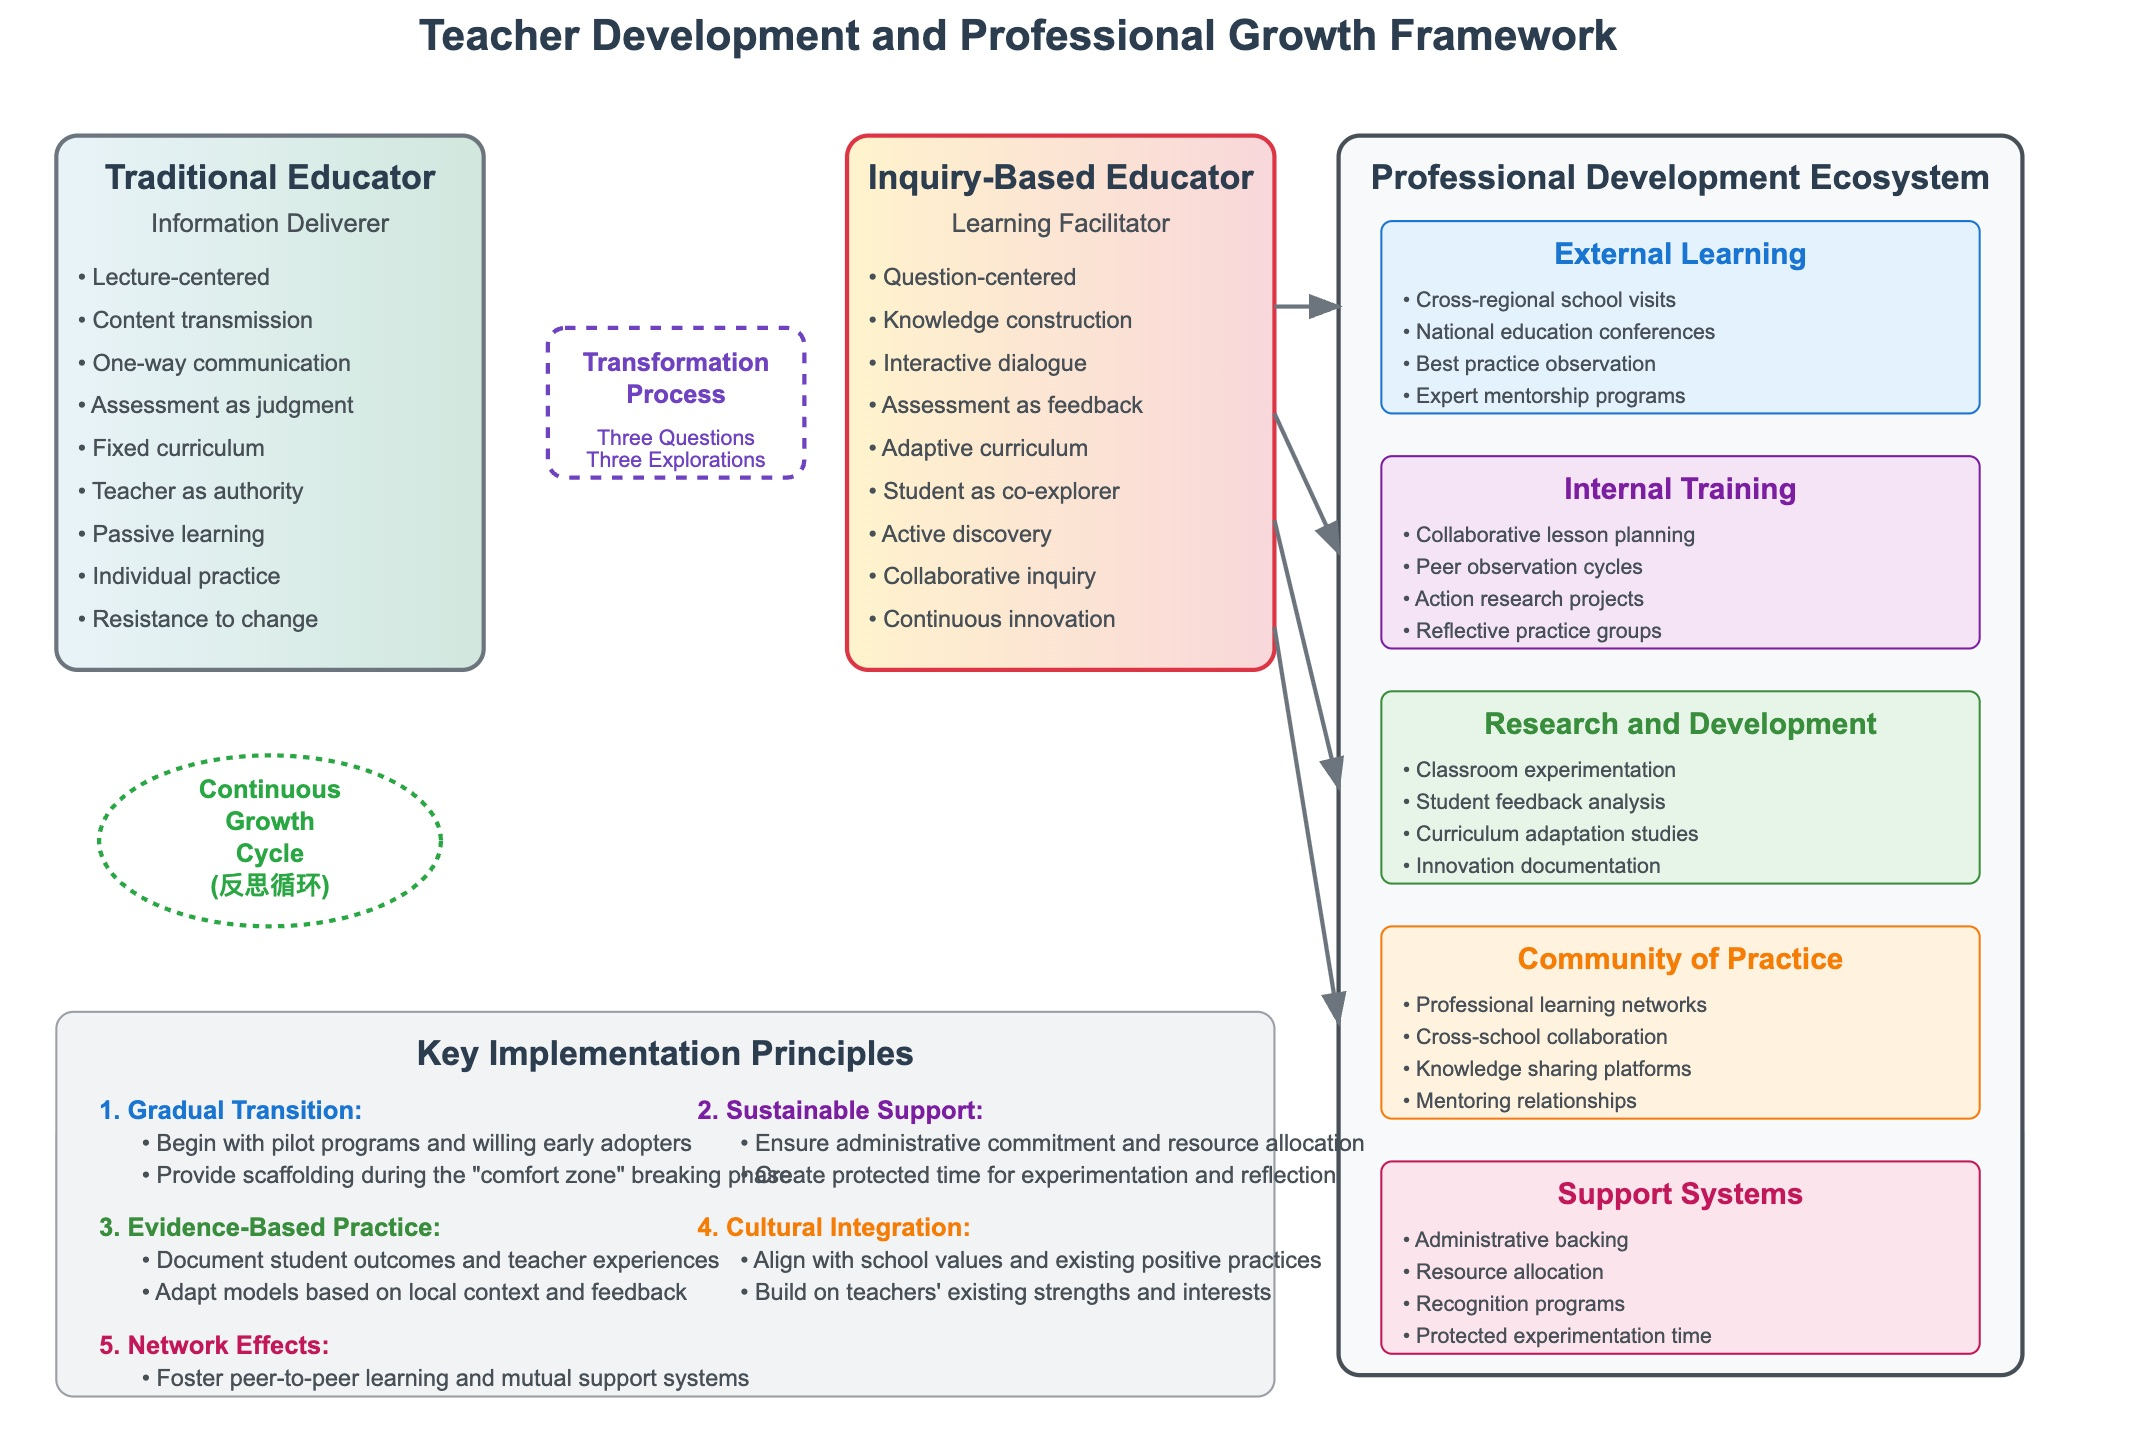
\includegraphics[keepaspectratio]{_resources/images/Ch7-TransformationFramework.jpg}}

\subsection{Internal Training
Programs}\label{internal-training-programs}

While external learning provides inspiration and exposure to new
possibilities, internal training programs offer the sustained support
necessary for deep professional transformation. Effective internal
programs are characterized by their responsiveness to local contexts,
their integration with ongoing school improvement efforts, and their
attention to the gradual nature of meaningful change.

Successful internal training programs often employ a coaching model that
pairs experienced inquiry-based practitioners with teachers new to the
approach. This mentoring relationship provides ongoing support,
immediate feedback, and gradual release of responsibility as new
practitioners develop confidence and competence. The coaching model
recognizes that learning to teach differently is a complex process that
unfolds over time through repeated practice and reflection.

Professional learning communities within schools create opportunities
for collaborative learning and shared problem-solving. When teachers
regularly engage in examining student work, analyzing teaching
practices, and discussing pedagogical challenges, they develop the
habits of mind necessary for continuous improvement. These communities
become laboratories for experimentation and refinement of inquiry-based
approaches.

Action research projects allow teachers to systematically investigate
their own practice while implementing new approaches. By collecting data
on student learning, reflecting on teaching decisions, and adjusting
practices based on evidence, teachers develop both practical skills and
research mindsets that support ongoing professional growth.

\section{Overcoming Resistance and Building
Confidence}\label{overcoming-resistance-and-building-confidence}

\subsection{Addressing Pedagogical
Anxiety}\label{addressing-pedagogical-anxiety}

The transition to inquiry-based teaching often generates significant
anxiety among educators who have achieved success with traditional
approaches. This anxiety is understandable and rational---teachers are
being asked to abandon familiar practices that have served them well in
favor of approaches that initially feel uncertain and risky. Effective
professional development programs acknowledge this anxiety and provide
structured support for working through it.

Common sources of anxiety include fear of losing classroom control when
students become more active participants in their learning, concern
about covering required curriculum content when inquiry processes take
longer than direct instruction, and worry about maintaining academic
standards when assessment practices must change to align with new
learning goals. These concerns reflect legitimate challenges that
require thoughtful response rather than dismissal.

Building confidence requires providing teachers with safe spaces to
experiment with new approaches, opportunities to observe successful
implementation by peers, and gradual introduction of inquiry-based
practices rather than wholesale transformation. Many successful reform
efforts begin with small-scale implementations that allow teachers to
experience success before expanding their use of inquiry-based
approaches.

\subsection{Creating Supportive Learning
Environments}\label{creating-supportive-learning-environments}

Professional development environments must model the inquiry-based
approaches they seek to promote. When teachers experience learning
through exploration, questioning, and collaborative problem-solving,
they develop both skills and dispositions necessary for implementing
similar approaches with their students. This alignment between
professional development methodology and desired classroom practices
reinforces learning and builds authentic understanding.

Psychological safety becomes paramount in professional development
contexts where teachers are asked to take risks and potentially make
mistakes as they learn new approaches. Administrators and professional
development leaders must create environments where experimentation is
encouraged, failures are treated as learning opportunities, and teachers
feel supported in their growth rather than evaluated or judged.

Peer collaboration and shared leadership in professional development
activities help distribute expertise and create multiple sources of
support. When teachers take responsibility for leading aspects of their
own professional learning, they develop ownership and investment in the
transformation process while building capacity for sustained
improvement.

\section{Sustainable Growth Models}\label{sustainable-growth-models}

\subsection{Continuous Learning
Cycles}\label{continuous-learning-cycles}

Sustainable professional development recognizes that learning to teach
through inquiry is an ongoing process rather than a discrete training
event. Effective programs establish cycles of learning that include
planning, implementation, reflection, and refinement. These cycles
mirror the inquiry processes that teachers are learning to facilitate
with their students.

Regular reflection protocols help teachers examine their practice
systematically, identify areas for growth, and set goals for continued
development. These protocols might include lesson analysis frameworks,
student learning assessments, or peer observation systems that provide
structured opportunities for examining teaching effectiveness.

Documentation and portfolio development allow teachers to track their
growth over time while creating resources for supporting colleagues who
are earlier in their transformation journey. When teachers maintain
records of their learning, including challenges faced and strategies
developed, they contribute to institutional knowledge while reinforcing
their own professional development.

\subsection{Building Internal
Capacity}\label{building-internal-capacity}

Long-term sustainability requires developing internal capacity for
supporting ongoing professional growth. This means identifying and
developing teacher leaders who can provide coaching and mentoring for
colleagues, creating systems for sharing effective practices within and
across schools, and establishing structures for continuous program
improvement.

Teacher leadership development involves more than simply identifying
effective practitioners. It requires providing potential leaders with
skills in adult learning, coaching methodologies, and change management.
These teacher leaders must understand not only how to implement
inquiry-based teaching effectively but also how to support others
through the complex process of professional transformation.

Knowledge management systems help institutions capture and share the
wisdom developed through reform implementation. When schools create
repositories of effective practices, common challenges and solutions,
and resources for supporting implementation, they build organizational
capacity for sustained improvement that transcends individual personnel
changes.

\section{Assessment and Evaluation of Professional
Growth}\label{assessment-and-evaluation-of-professional-growth}

\subsection{Measuring Transformation}\label{measuring-transformation}

Assessing teacher development in inquiry-based approaches requires
evaluation frameworks that go beyond traditional measures of teaching
effectiveness. While student achievement data remains important, it must
be supplemented with measures that capture the complex processes
involved in facilitating inquiry-based learning.

Classroom observation protocols must be redesigned to focus on the
quality of questioning, the degree of student engagement in authentic
problems, and the effectiveness of scaffolding provided during inquiry
processes. These observations require trained evaluators who understand
inquiry-based teaching and can distinguish between surface-level
implementation and deep pedagogical transformation.

Self-assessment tools allow teachers to monitor their own development
while building metacognitive awareness of their teaching practices. When
teachers regularly reflect on their implementation of inquiry-based
approaches, they develop the self-monitoring capabilities necessary for
continuous improvement.

\subsection{Portfolio-Based
Documentation}\label{portfolio-based-documentation}

Professional portfolios provide rich documentation of teacher growth
over time while creating opportunities for reflective analysis.
Effective portfolios include lesson plans, student work samples,
reflection essays, and video documentation that demonstrate the
evolution of teaching practices and student learning outcomes.

Portfolio development processes should include regular review and
analysis sessions where teachers examine their documentation with
colleagues or mentors. These collaborative reviews provide opportunities
for shared learning while supporting individual growth through
structured reflection and feedback.

Digital portfolio platforms can facilitate sharing and collaboration
while providing tools for organizing and analyzing professional growth
documentation. When teachers can easily access and share their work with
colleagues, they contribute to collective learning while receiving
support for their individual development.

\section{Conclusion}\label{conclusion-4}

The transformation of teachers from information deliverers to learning
facilitators represents both the greatest challenge and the most
critical success factor in implementing inquiry-based education. This
transformation requires comprehensive professional development systems
that address both the technical aspects of new pedagogical approaches
and the emotional and psychological dimensions of significant
professional change.

Successful teacher development programs recognize that meaningful change
occurs gradually through sustained support, repeated practice, and
continuous reflection. They provide multiple pathways for learning while
maintaining focus on the ultimate goal of improved student learning
through inquiry-based approaches.

The evidence from regional reform initiatives demonstrates that when
teachers receive appropriate support for professional transformation,
they can successfully implement inquiry-based approaches that
significantly enhance student learning. However, this transformation
requires institutional commitment to long-term professional development
processes that honor the complexity of changing deeply held beliefs and
practices about teaching and learning.

As educational systems continue to evolve in response to changing
societal needs and technological possibilities, the capacity to support
teacher development will remain a critical determinant of reform
success. The frameworks and strategies outlined in this chapter provide
roadmaps for supporting educators through the challenging but ultimately
rewarding process of professional transformation that inquiry-based
education demands.

\bookmarksetup{startatroot}

\chapter{Avoiding Common Pitfalls in
Reform}\label{avoiding-common-pitfalls-in-reform}

\section{Introduction}\label{introduction-6}

Educational reform initiatives, despite the best intentions of their
architects, frequently encounter predictable obstacles that can derail
even the most thoughtfully designed transformation efforts. The Chinese
educational reform literature identifies several critical failure modes
that plague curriculum change initiatives: formalism (形式主义: xíngshì
zhǔyì), borrowed solutions without adaptation (拿来主义: nálái zhǔyì),
blind rapid advancement (盲目跃进: mángmù yuèjìn), and superficial
innovation (盲目创新: mángmù chuàngxīn). Understanding these pitfalls
and developing systematic approaches to avoid them represents a crucial
competency for educational leaders committed to authentic
transformation.

The stakes of avoiding these pitfalls extend beyond mere implementation
efficiency. When reform efforts fail due to preventable errors, the
resulting institutional skepticism can create lasting resistance to
future change initiatives, effectively inoculating organizations against
beneficial transformation for years or even decades. More importantly,
failed reforms waste the precious resource of educator goodwill and
student opportunity, making the development of robust failure-prevention
frameworks an ethical imperative for reform leaders.

\section{The Formalism Trap: When Process Becomes
Performance}\label{the-formalism-trap-when-process-becomes-performance}

Formalism represents perhaps the most insidious threat to authentic
educational reform. This pitfall manifests when organizations focus
disproportionately on the visible symbols and procedures of reform while
neglecting the underlying pedagogical transformation that such
procedures are meant to facilitate. Educational systems caught in
formalism traps often exhibit impressive compliance with reform
protocols while maintaining fundamentally unchanged instructional
practices.

The formalism trap typically emerges from misaligned incentive
structures within educational bureaucracies. When administrators
evaluate reform progress primarily through easily quantifiable metrics
such as training attendance, document completion, or classroom
observation checklists, teachers rationally respond by optimizing for
these measures rather than for genuine pedagogical improvement. This
dynamic creates what might be termed ``reform theater''---elaborate
performances of change that mask continued adherence to traditional
practices.

Consider the implementation of inquiry-based learning initiatives that
become reduced to mandatory question-asking quotas or prescribed
discussion formats. Teachers may dutifully implement the structural
elements of inquiry pedagogy while maintaining traditional authoritarian
classroom relationships and didactic information transmission. Students
learn to perform the expected behaviors of inquiry learners without
developing genuine critical thinking capabilities or intellectual
autonomy.

The prevention of formalism requires what systems theorists would
recognize as a shift from first-order to second-order change.
First-order change modifies surface behaviors and procedures while
leaving underlying assumptions and power structures intact. Second-order
change transforms the fundamental operating principles and belief
systems that generate observable behaviors. Educational leaders must
therefore design reform evaluation systems that can detect and reward
second-order changes in teacher practice and student engagement.

Effective anti-formalism strategies begin with the recognition that
authentic reform requires transformation of educator mental models
rather than mere compliance with new procedures. This necessitates
investment in deep professional development experiences that help
teachers understand the theoretical foundations and practical
implications of proposed changes. As discussed in Chapter 7, such
development cannot be accomplished through brief workshops or mandate
delivery, but requires sustained engagement with both content knowledge
and pedagogical reflection.

\section{The Borrowing Trap: Inappropriate Adaptation of External
Models}\label{the-borrowing-trap-inappropriate-adaptation-of-external-models}

The second major pitfall facing reform initiatives involves the
uncritical adoption of educational models developed in different
contexts without adequate adaptation to local conditions. This
``borrowing trap'' often emerges from legitimate desires to learn from
successful innovations while lacking the analytical frameworks necessary
to determine which elements of external models are transferable and
which require significant modification.

Educational borrowing becomes problematic when reform leaders assume
that successful practices are universally applicable regardless of
cultural, institutional, or resource contexts. The globalization of
educational discourse has created unprecedented opportunities for
cross-pollination of pedagogical innovations, but it has also generated
pressure to adopt fashionable reform models without sufficient
consideration of implementation requirements or contextual fit.

The borrowing trap manifests in several distinct patterns. Surface-level
borrowing involves adopting the visible structures and procedures of
successful programs while missing the underlying principles that make
them effective. For example, schools might implement the scheduling and
grouping arrangements associated with project-based learning without
developing the teacher capabilities or student preparation necessary to
make such arrangements productive.

Cultural borrowing failures occur when educational models developed
within specific cultural contexts are transplanted to environments with
fundamentally different assumptions about learning, authority, and
knowledge. The inquiry-based pedagogies discussed throughout this book,
for instance, rest on particular assumptions about student agency and
intellectual authority that may conflict with educational cultures
emphasizing respect for teacher expertise and established knowledge
hierarchies.

Resource borrowing failures emerge when schools attempt to implement
programs requiring significant human, technological, or financial
resources without ensuring adequate support systems. Many
technology-enhanced learning initiatives fail not because of pedagogical
inadequacy but because schools lack the technical infrastructure,
teacher training, or ongoing support necessary for sustainable
implementation.

Prevention of borrowing traps requires what might be termed
``intelligent adaptation''---systematic processes for analyzing external
models, identifying their essential principles, and redesigning
implementation approaches that honor those principles while fitting
local constraints and opportunities. This process begins with careful
analysis of the underlying theories and mechanisms that make borrowed
models effective in their original contexts.

Intelligent adaptation also requires honest assessment of local capacity
and constraints. Educational leaders must resist the temptation to
assume that enthusiasm and good intentions can overcome significant
resource or capability gaps. Instead, they must develop realistic
implementation timelines that allow for gradual capacity building and
iterative refinement of borrowed practices.

\section{The Rush Trap: Blind Rapid
Advancement}\label{the-rush-trap-blind-rapid-advancement}

The third critical pitfall involves attempts to accelerate reform
implementation beyond the pace that organizational learning and cultural
change can sustain. This ``rush trap'' typically emerges from legitimate
concerns about student opportunity costs and institutional urgency, but
it often produces counterproductive outcomes that ultimately delay
authentic transformation.

Rapid advancement becomes problematic when it outpaces the development
of necessary human capabilities and institutional supports. Educational
reform requires complex learning processes that cannot be artificially
accelerated without compromising quality and sustainability. Teachers
need time to internalize new pedagogical approaches, administrators need
time to develop supportive evaluation and resource allocation systems,
and students need time to adapt to changed expectations and
opportunities.

The rush trap often manifests as premature scaling of pilot programs
before they have been adequately tested and refined. Organizations
experiencing early success with small-scale innovations may feel
pressure to implement them system-wide before understanding the full
range of implementation challenges or developing robust support systems.
This pattern frequently leads to diluted versions of originally
effective practices and widespread implementation failures that damage
institutional confidence in reform initiatives.

Another common manifestation involves attempting to implement multiple
major changes simultaneously without considering the cognitive and
emotional demands such changes place on educators. Teachers have limited
capacity for processing fundamental changes to their professional
practice, and organizations that overwhelm this capacity often find that
all changes are implemented superficially rather than any being
implemented deeply.

Prevention of rush traps requires what organizational learning theorists
describe as ``dynamic pacing''---the ability to calibrate reform
timelines to organizational learning capacity rather than external
pressure or artificial deadlines. This involves developing sophisticated
understanding of the change process stages that educators must navigate
and designing implementation schedules that provide adequate time for
each stage.

Effective pacing strategies also recognize that different aspects of
reform may proceed at different rates. Structural changes such as
scheduling modifications or resource allocation adjustments may be
implemented relatively quickly, while pedagogical changes requiring new
teacher competencies may require years of sustained development. Reform
leaders must resist pressure to demonstrate rapid progress in all
dimensions simultaneously and instead focus on creating conditions for
deep, sustainable change.

\section{The Innovation Trap: Blind Creativity Without
Foundation}\label{the-innovation-trap-blind-creativity-without-foundation}

The fourth major pitfall involves excessive emphasis on novelty and
creativity at the expense of proven pedagogical principles and empirical
evidence. This ``innovation trap'' emerges from cultures that valorize
change for its own sake rather than change directed toward clearly
defined educational outcomes.

Blind innovation becomes problematic when schools pursue novel
approaches without adequate consideration of their theoretical
foundations or empirical support. The contemporary emphasis on
innovation in educational discourse can create pressure to develop
unique solutions even when effective approaches already exist and simply
require competent implementation.

The innovation trap often manifests as ``solution churn''---rapid
cycling through multiple reform initiatives without allowing sufficient
time for any to be properly implemented and evaluated. Schools caught in
this pattern may adopt new programs every few years in response to
disappointing results from previous innovations, not recognizing that
their evaluation timeframes are insufficient for detecting genuine
improvement.

Another manifestation involves what might be termed ``innovation
theater''---the adoption of superficially novel practices that appear
innovative but lack substantive pedagogical improvement. Technology
integration initiatives that focus on device acquisition rather than
pedagogical transformation exemplify this pattern, as do project-based
learning implementations that maintain traditional assessment and
authority structures while changing only surface features of student
activity.

Prevention of innovation traps requires grounding all change initiatives
in clearly articulated theories of learning and empirical evidence of
effectiveness. This does not preclude genuine innovation, but it ensures
that creative efforts are directed toward solving real pedagogical
problems rather than creating artificial novelty.

Effective innovation frameworks also emphasize the importance of what
educational researchers term ``productive failure''---systematic
experimentation that generates useful learning even when specific
innovations prove unsuccessful. Such frameworks require robust
evaluation systems that can distinguish between innovations that fail
due to implementation problems and those that fail due to fundamental
design flaws.

\section{Developing Institutional
Immunity}\label{developing-institutional-immunity}

The prevention of these common pitfalls requires more than awareness and
good intentions. Educational organizations must develop systematic
frameworks for detecting and preventing the conditions that generate
formalism, inappropriate borrowing, premature acceleration, and blind
innovation.

Effective prevention frameworks begin with clear articulation of reform
theories and intended outcomes. Organizations that cannot clearly
explain why specific changes should produce desired improvements lack
the analytical foundation necessary for distinguishing authentic
progress from mere activity. Such articulation requires engagement with
relevant research literature and explicit consideration of causal
mechanisms linking proposed changes to desired outcomes.

Prevention frameworks also require robust feedback systems that can
detect early warning signs of pitfall development. These systems must be
sensitive to both quantitative indicators of implementation progress and
qualitative indicators of educator experience and student response. The
development of such systems represents a significant investment in
organizational learning capability that pays dividends across multiple
reform initiatives.

Perhaps most importantly, prevention frameworks must address the
underlying organizational and cultural factors that make pitfalls
attractive. Formalism thrives in environments with misaligned incentives
and superficial evaluation systems. Inappropriate borrowing flourishes
when organizations lack confidence in their analytical capabilities.
Rush behaviors emerge from anxiety about performance pressure and
insufficient understanding of change processes. Blind innovation
develops in cultures that value novelty over effectiveness.

\section{Conclusion}\label{conclusion-5}

The avoidance of common reform pitfalls represents a learnable
organizational competency that can dramatically improve the success rate
of educational transformation initiatives. By understanding the
systematic patterns through which formalism, inappropriate borrowing,
premature acceleration, and blind innovation develop, educational
leaders can design prevention strategies that address root causes rather
than merely treating symptoms.

The frameworks discussed in this chapter require significant investment
in organizational learning capabilities and cultural development.
However, such investments represent essential infrastructure for
sustainable educational improvement rather than optional enhancements to
reform initiatives. Organizations that develop robust pitfall prevention
capabilities position themselves for sustained success across multiple
change initiatives rather than repeated cycles of reform disappointment.

The next chapter will examine how these prevention frameworks can be
integrated with comprehensive assessment and evaluation systems that
support authentic educational transformation while avoiding the
measurement problems that contribute to reform pitfalls.

\bookmarksetup{startatroot}

\chapter{Assessment and Evaluation
Systems}\label{assessment-and-evaluation-systems}

\section{Introduction: The Assessment Paradigm
Shift}\label{introduction-the-assessment-paradigm-shift}

The transformation from traditional instructional models to
inquiry-based learning necessitates a fundamental reconceptualization of
how we measure student progress and educational effectiveness. As
discussed in Chapter 3's strategic top-level design principles,
assessment systems must align with the core philosophy of believing in
students and cultivating their questioning abilities. Traditional
testing regimes, designed for passive knowledge consumption, become not
merely inadequate but actively counterproductive when applied to
inquiry-driven educational environments.

The challenge lies in developing evaluation frameworks that capture the
dynamic, non-linear nature of inquiry-based learning while maintaining
the rigor and accountability demanded by educational stakeholders. This
chapter examines how assessment systems can evolve to support rather
than constrain the ``Three Questions, Three Explorations'' methodology
explored in Chapter 4, creating feedback loops that reinforce critical
thinking and authentic learning rather than memorization and compliance.

\section{Theoretical Foundations of Inquiry-Based
Assessment}\label{theoretical-foundations-of-inquiry-based-assessment}

Assessment in inquiry-based environments must operate from fundamentally
different assumptions about learning and knowledge construction. Where
traditional assessment treats knowledge as a fixed commodity to be
accumulated and regurgitated, inquiry-based assessment recognizes
knowledge as dynamic, contextual, and co-constructed through the
interaction between learner, content, and community.

This shift demands what we might term \emph{processual assessment}
(過程評估; guòchéng pínggū) --- evaluation that captures the unfolding
of thinking rather than merely its endpoints. Such assessment recognizes
that the quality of questions students generate often reveals deeper
understanding than their ability to answer predetermined queries. When
students engage in authentic inquiry, their learning trajectories become
inherently unpredictable, requiring assessment approaches that can
accommodate emergence and serendipity rather than demanding strict
adherence to predetermined outcomes.

The epistemological foundation for such assessment draws from
constructivist learning theory, which posits that learners actively
build understanding through interaction with their environment rather
than passively receiving transmitted information. This perspective
demands assessment practices that reveal not what students know in
isolation, but how they think, how they approach problems, and how they
construct meaning from experience.

\section{Designing Assessment Systems for Critical
Thinking}\label{designing-assessment-systems-for-critical-thinking}

Effective assessment of critical thinking requires moving beyond the
measurement of discrete cognitive skills toward evaluation of thinking
as an integrated, contextual practice. Critical thinking manifests not
as a collection of techniques but as a disposition toward questioning
assumptions, examining evidence, considering alternative perspectives,
and drawing reasoned conclusions.

Assessment frameworks must therefore capture what might be called
\emph{thinking in action} rather than thinking about thinking. This
requires observational protocols that document how students approach
unfamiliar problems, how they revise their understanding when presented
with contradictory evidence, and how they collaborate to construct
shared understanding. Such documentation necessarily becomes more
qualitative and narrative-based, moving away from the quantitative
precision of traditional metrics toward rich description of learning
processes.

One promising approach involves the development of \emph{thinking
portfolios} that document student reasoning over time. These portfolios
capture not merely final products but the evolution of student thinking,
including false starts, revised hypotheses, and breakthrough moments.
The portfolio becomes a space for metacognitive reflection, where
students examine their own thinking processes and develop greater
awareness of their learning strategies.

Assessment rubrics for critical thinking must acknowledge the situated
nature of reasoning. A student's critical thinking abilities may
manifest differently across domains, and assessment systems must be
sensitive to these variations while still maintaining coherent
standards. This suggests the need for domain-specific assessment
criteria that nonetheless share common elements related to evidence
evaluation, perspective-taking, and logical reasoning.

\section{Evaluating Problem-Solving
Abilities}\label{evaluating-problem-solving-abilities}

Problem-solving assessment in inquiry-based environments faces the
challenge of evaluating a fundamentally creative and unpredictable
process using necessarily structured evaluation tools. Authentic
problem-solving involves navigating uncertainty, generating novel
approaches, and persisting through setbacks --- qualities that resist
easy quantification.

Effective problem-solving assessment must therefore focus on
\emph{adaptive expertise} rather than routine expertise. Where routine
expertise involves the efficient application of well-learned procedures,
adaptive expertise involves the flexible application of knowledge and
skills to novel situations. Assessment of adaptive expertise requires
presenting students with problems that cannot be solved through
memorized algorithms or procedures, demanding instead the creative
application of underlying principles.

Performance assessment becomes central to evaluating problem-solving
abilities. Students must be observed and evaluated while engaged in
authentic problem-solving activities rather than while responding to
abstract representations of problems. This observational approach allows
assessors to document student strategies, their responses to obstacles,
their ability to revise approaches when initial strategies prove
inadequate, and their persistence in the face of difficulty.

The assessment of collaborative problem-solving presents additional
complexities. When students work together to solve problems, individual
contributions become difficult to isolate, yet the collaborative
dimension represents a crucial aspect of real-world problem-solving.
Assessment frameworks must develop approaches for evaluating both
individual contributions to collaborative efforts and the emergent
properties of group problem-solving that exceed the sum of individual
capabilities.

Documentation of problem-solving processes might employ video analysis,
thinking-aloud protocols, and digital portfolios that capture the
evolution of student thinking over extended time periods. Such
documentation provides rich data for both formative feedback to students
and summative evaluation of program effectiveness.

\section{Student Engagement Metrics}\label{student-engagement-metrics}

Traditional measures of student engagement, such as time-on-task or
homework completion rates, prove inadequate for capturing the quality of
engagement characteristic of inquiry-based learning environments.
Authentic engagement in inquiry involves intellectual risk-taking,
sustained attention to complex problems, and intrinsic motivation to
pursue understanding --- qualities that resist simple quantification.

Engagement assessment must distinguish between compliance and authentic
intellectual involvement. Students may demonstrate high levels of task
completion while remaining intellectually disengaged, following
procedures without understanding or caring about outcomes. Conversely,
deeply engaged students may appear non-compliant with traditional
measures while pursuing self-directed investigations that demonstrate
profound intellectual commitment.

Observable indicators of authentic engagement include the quality of
questions students generate, their willingness to revise initial ideas
when presented with new evidence, their persistence when facing
challenging problems, and their ability to make connections between
current learning and previous experience. These indicators require
systematic observation and documentation rather than simple measurement.

Technology can provide valuable tools for engagement assessment through
learning analytics that track student interactions with digital learning
environments. Patterns of exploration, revision, and collaboration in
digital spaces can reveal engagement levels that might not be apparent
through traditional observation. However, such data must be interpreted
carefully, recognizing that meaningful engagement may not always
correlate with high levels of digital activity.

Student self-assessment of engagement becomes particularly valuable in
inquiry-based environments, where learners develop greater awareness of
their own learning processes. Self-reflection tools that prompt students
to examine their own motivation, curiosity, and intellectual investment
provide insights into engagement that external observation cannot
capture.

\section{Formative vs.~Summative Assessment
Strategies}\label{formative-vs.-summative-assessment-strategies}

The distinction between formative and summative assessment becomes
particularly crucial in inquiry-based learning environments, where the
unpredictable nature of authentic learning makes it difficult to specify
in advance exactly what students should know or be able to do at
particular points in time.

Formative assessment in inquiry-based environments serves primarily to
support ongoing learning rather than to measure achievement against
predetermined standards. Such assessment focuses on helping students
understand their own thinking processes, identify areas for further
investigation, and develop metacognitive awareness of their learning
strategies. The feedback provided through formative assessment must be
timely, specific, and actionable, helping students adjust their
approaches while engaged in learning activities.

Effective formative assessment in inquiry-based environments often takes
the form of learning conversations between teachers and students, where
the focus shifts from evaluation to exploration. Teachers ask questions
that prompt student reflection: ``What evidence supports your
conclusion? What questions does this raise for you? How does this
connect to what you learned previously?'' Such conversations model the
questioning disposition central to inquiry-based learning while
providing valuable diagnostic information about student understanding.

Peer assessment becomes particularly valuable in inquiry-based
environments, where students learn to evaluate each other's thinking and
provide constructive feedback. This process develops critical evaluation
skills while distributing the assessment workload and providing students
with multiple perspectives on their work. However, peer assessment
requires careful scaffolding to ensure that feedback is constructive and
that students develop appropriate criteria for evaluation.

Summative assessment in inquiry-based environments faces the challenge
of evaluating learning that may not conform to predetermined
trajectories. Traditional summative assessments, designed to measure
mastery of specified content or skills, may miss the most significant
learning that occurs through authentic inquiry. Alternative approaches
to summative assessment might include portfolio reviews, exhibition of
learning, or demonstration projects that allow students to showcase
their learning in flexible formats.

The timing of summative assessment also requires reconsideration in
inquiry-based environments. Rather than occurring at predetermined
intervals, summative assessment might occur when students feel ready to
demonstrate their learning or when natural culmination points emerge
from inquiry processes. This approach requires greater flexibility from
educational systems while maintaining accountability for learning
outcomes.

\section{Technology Integration in
Assessment}\label{technology-integration-in-assessment}

Digital technologies offer both opportunities and challenges for
assessment in inquiry-based learning environments. On one hand,
technology can provide sophisticated tools for capturing and analyzing
learning processes that would be impossible to document through
traditional means. On the other hand, the integration of technology in
assessment raises questions about privacy, equity, and the potential for
technological tools to constrain rather than enhance learning.

Learning analytics represent one of the most promising applications of
technology in assessment, providing detailed data about student
interactions with digital learning environments. Patterns of
exploration, collaboration, and revision can reveal insights into
learning processes that external observation might miss. However, the
interpretation of such data requires sophisticated understanding of both
learning processes and data analysis techniques.

Adaptive assessment systems can adjust to student responses in
real-time, providing more precise measurements of student abilities
while reducing testing time and student fatigue. Such systems can
provide immediate feedback to students and teachers while generating
detailed profiles of student strengths and areas for growth. However,
adaptive systems require careful design to ensure that they support
rather than constrain inquiry-based learning.

Digital portfolios provide powerful tools for documenting learning over
time, allowing students to collect, organize, and reflect on their work
in multimedia formats. Such portfolios can capture not only final
products but also process documentation, including draft work,
reflection pieces, and collaborative exchanges. The digital format
enables easy sharing and collaboration while providing sophisticated
tools for analysis and evaluation.

Virtual and augmented reality technologies offer new possibilities for
performance assessment by creating immersive environments where students
can demonstrate learning in realistic contexts. Such environments can
provide standardized yet authentic assessment experiences that would be
impossible to create in physical spaces.

However, technology integration in assessment must be approached
thoughtfully, recognizing that technological sophistication does not
necessarily improve assessment validity or usefulness. The fundamental
questions remain: What are we trying to assess? How can we best capture
evidence of that learning? How can assessment support further learning?
Technology should enhance rather than drive assessment design.

\section{Cultural and Contextual
Considerations}\label{cultural-and-contextual-considerations}

Assessment systems must be sensitive to the cultural contexts in which
learning occurs, recognizing that different communities may have
different values, communication styles, and ways of demonstrating
knowledge. What counts as evidence of learning, how that evidence should
be communicated, and who has authority to evaluate learning may vary
significantly across cultural contexts.

In many traditional cultures, knowledge demonstration occurs through
storytelling, practical application, or community contribution rather
than through individual performance on decontextualized tasks.
Assessment systems in diverse communities must incorporate multiple ways
of knowing and showing, ensuring that all students have opportunities to
demonstrate their learning in culturally meaningful ways.

Language differences present particular challenges for assessment in
inquiry-based environments, where much of the evidence of learning
emerges through verbal communication and written reflection. Students
who are developing proficiency in the language of instruction may
demonstrate sophisticated thinking that is not fully captured by
linguistically demanding assessment tasks. Assessment systems must
distinguish between language proficiency and conceptual understanding,
providing multiple modalities for students to demonstrate their
learning.

Socioeconomic factors also influence assessment validity, as students
from different backgrounds may have varying access to experiences,
technologies, and cultural capital that assessment tasks assume. Equity
in assessment requires careful attention to potential bias in task
design, ensuring that assessment focuses on the constructs of interest
rather than on background knowledge or experiences that may not be
equally available to all students.

The communalistic values present in many cultures may conflict with the
individualistic assumptions underlying traditional assessment
approaches. In cultures that emphasize collective achievement and group
harmony, individual performance assessment may not align with cultural
values and may not capture the most meaningful aspects of learning.
Assessment systems must be flexible enough to accommodate different
cultural orientations while maintaining coherent standards for learning.

\section{Implementation Challenges and
Solutions}\label{implementation-challenges-and-solutions}

The transition from traditional assessment systems to inquiry-based
evaluation approaches faces significant practical, political, and
institutional challenges. Existing accountability systems, standardized
testing requirements, and stakeholder expectations may conflict with the
assessment approaches most appropriate for inquiry-based learning.

Professional development for educators represents one of the most
significant implementation challenges. Teachers who have been trained in
traditional assessment approaches may lack the knowledge and skills
necessary to design and implement assessment for inquiry-based learning.
Such professional development must be ongoing and practice-based,
providing teachers with opportunities to experiment with new assessment
approaches while receiving feedback and support.

Parent and community understanding of new assessment approaches requires
careful attention. When assessment moves away from familiar formats like
tests and grades toward portfolios, exhibitions, and narrative
evaluation, parents may question whether rigorous evaluation is
occurring. Communication about the purposes and methods of inquiry-based
assessment must be clear, ongoing, and responsive to community concerns.

Institutional systems for recording, reporting, and analyzing assessment
data may require significant modification to accommodate assessment
approaches that generate qualitative, narrative, and portfolio-based
evidence rather than numerical scores. Information systems must be
flexible enough to handle diverse forms of evidence while still
providing useful data for decision-making.

Scaling assessment innovations from individual classrooms to
institutional and system levels presents additional challenges.
Assessment approaches that work well in single classrooms may prove
difficult to implement consistently across schools or districts.
Successful scaling requires attention to training, resources, and
systemic support for assessment innovation.

Time represents a persistent challenge for inquiry-based assessment, as
meaningful evaluation of complex learning processes requires significant
investment from teachers and students. Schools must consider how to
restructure time allocation to accommodate more intensive assessment
approaches while maintaining coverage of required content and skills.

\section{Building Sustainable Assessment
Systems}\label{building-sustainable-assessment-systems}

Sustainability in inquiry-based assessment requires creating systems
that can maintain quality and coherence over time while adapting to
changing contexts and evolving understanding of effective practice. Such
sustainability depends on institutional commitment, ongoing professional
development, and systematic attention to continuous improvement.

The development of assessment literacy among all stakeholders becomes
crucial for sustainability. Teachers, administrators, students, parents,
and community members must develop understanding of inquiry-based
assessment approaches and their value for supporting deep learning. This
assessment literacy cannot be achieved through one-time training but
requires ongoing engagement and education.

Systematic documentation and evaluation of assessment practices enables
continuous improvement and provides evidence of effectiveness for
skeptical stakeholders. Schools and districts implementing inquiry-based
assessment must collect and analyze data about the impact of their
assessment approaches on student learning, teacher practice, and
institutional culture.

Collaboration among educators implementing inquiry-based assessment
creates communities of practice that can support innovation and
problem-solving. Such collaboration may occur within institutions,
across districts, or through professional networks that connect
educators working on similar challenges.

Financial sustainability requires realistic assessment of the costs
associated with inquiry-based assessment and creative approaches to
funding ongoing implementation. While some aspects of inquiry-based
assessment may require additional resources, others may prove more
cost-effective than traditional approaches, particularly when
considering the long-term impact on student learning and engagement.

\section{Conclusion: Assessment as Learning
Support}\label{conclusion-assessment-as-learning-support}

The transformation of assessment systems to support inquiry-based
learning represents more than a technical challenge; it requires
fundamental reconsideration of the purposes and methods of educational
evaluation. As outlined throughout this chapter, effective assessment in
inquiry-based environments must move beyond measurement toward learning
support, beyond standardization toward responsive adaptation, and beyond
individual performance toward collaborative knowledge construction.

The assessment approaches described here align with the
consensus-building and top-level design principles discussed in earlier
chapters, recognizing that assessment systems both reflect and shape
educational values and practices. When assessment focuses on curiosity,
critical thinking, and collaborative problem-solving, it sends clear
messages to students, teachers, and communities about what kinds of
learning are most valued.

The journey toward effective inquiry-based assessment requires patience,
persistence, and willingness to learn from both successes and failures.
As Chapter 10 will explore in detail, sustaining educational innovation
requires systematic attention to the conditions that support long-term
change. Assessment systems that truly support inquiry-based learning
cannot be implemented overnight but must evolve through careful
experimentation, reflection, and continuous improvement.

The ultimate goal of inquiry-based assessment is not merely to measure
learning more accurately but to create assessment experiences that are
themselves educative, helping students develop the metacognitive
awareness, critical thinking skills, and collaborative capabilities they
will need for lifelong learning. When assessment becomes
indistinguishable from learning, we will have achieved the integration
of evaluation and education that inquiry-based approaches demand.

\bookmarksetup{startatroot}

\chapter{Sustaining Long-Term Educational
Change}\label{sustaining-long-term-educational-change}

\section{Introduction}\label{introduction-7}

The implementation of inquiry-based learning represents only the
beginning of a transformational journey. While the initial phases of
educational reform often generate excitement and visible progress, the
true test lies in sustaining these changes over time. Historical
analysis of educational innovations reveals a sobering pattern:
promising reforms frequently fade within three to five years, leaving
institutions to cycle through successive waves of change initiatives
without achieving lasting transformation.

The challenge of sustainability extends beyond maintaining specific
pedagogical practices. It encompasses the preservation of institutional
memory, the cultivation of adaptive capacity, and the development of
self-reinforcing systems that continue to evolve while maintaining core
principles. This chapter examines the mechanisms through which
educational change becomes embedded in organizational DNA rather than
remaining dependent on individual champions or external mandates.

\section{The Architecture of Sustainable
Change}\label{the-architecture-of-sustainable-change}

Sustainable educational transformation requires a shift from episodic
reform efforts to the development of what organizational theorists term
``learning organizations.'' In the context of inquiry-based education,
this means creating institutions that continuously adapt their practices
while maintaining fidelity to core principles of student-centered
learning and critical thinking development.

The foundation of such sustainability lies in establishing what
complexity scientists call ``emergent stability''---the capacity for
systems to maintain coherent patterns while adapting to changing
conditions. Unlike rigid adherence to prescribed methods, sustainable
inquiry-based education develops through the dynamic interaction of
stable core principles with flexible implementation strategies.

Research from the field of organizational psychology suggests that
lasting change occurs when three conditions converge: structural
modifications that reinforce desired behaviors, cultural shifts that
normalize new practices, and individual-level transformations that
internalize new ways of thinking. In educational contexts, this
translates to modifications in assessment systems, gradual shifts in
professional norms, and deep changes in teacher identity and practice.

\section{Creating Self-Reinforcing
Systems}\label{creating-self-reinforcing-systems}

The most robust approach to sustainability involves designing systems
that naturally reinforce inquiry-based practices rather than requiring
constant external pressure or oversight. These self-reinforcing
mechanisms operate at multiple organizational levels, from classroom
interactions to administrative policies.

At the classroom level, sustainable inquiry-based education emerges when
the pedagogical approach begins to generate its own momentum. Students
who develop questioning skills and critical thinking abilities create a
classroom dynamic that naturally supports continued inquiry. Teachers
report that once students internalize the expectation of active
engagement and intellectual curiosity, maintaining traditional
lecture-based formats becomes increasingly difficult and unsatisfying.

The development of teacher learning communities represents another
crucial self-reinforcing mechanism. When educators regularly collaborate
to refine inquiry-based practices, share challenges, and celebrate
successes, the professional culture begins to sustain itself. These
communities develop institutional knowledge that transcends individual
teacher turnover, creating repositories of practical wisdom that new
educators can access and contribute to.

Administrative systems also require redesign to support long-term
sustainability. Traditional evaluation frameworks that emphasize
standardized test scores and compliance with predetermined curricula
create pressures that undermine inquiry-based approaches. Sustainable
implementation requires the development of assessment systems that
measure the outcomes most valued in inquiry-based education: student
engagement, critical thinking development, and collaborative
problem-solving abilities.

\section{Institutional Memory and Knowledge
Management}\label{institutional-memory-and-knowledge-management}

One of the most significant threats to sustainable educational change
lies in the loss of institutional memory as personnel change over time.
Educational institutions often experience high turnover rates among both
teachers and administrators, leading to cyclical forgetting of hard-won
lessons and the erosion of reform initiatives.

Effective knowledge management systems capture not only the formal
procedures of inquiry-based education but also the tacit knowledge that
experienced practitioners develop through years of implementation. This
includes understanding of common student misconceptions, strategies for
handling resistance to new approaches, and techniques for adapting
general principles to specific contexts.

The documentation of implementation stories serves as a particularly
valuable form of institutional memory. These narratives capture the
journey of transformation, including the inevitable setbacks,
breakthrough moments, and gradual refinements that characterize
successful change processes. New faculty members benefit from
understanding not just what practices to implement, but how those
practices evolved and why certain approaches proved successful in their
specific context.

Mentorship programs that pair experienced inquiry-based educators with
newcomers provide another mechanism for preserving and transmitting
institutional knowledge. These relationships facilitate the transfer of
both explicit knowledge about pedagogical techniques and implicit
understanding of how to navigate the challenges of implementation within
the particular organizational culture.

\section{Building Adaptive Capacity}\label{building-adaptive-capacity}

Sustainable educational change requires institutions to develop what
resilience theorists call ``adaptive capacity''---the ability to adjust
practices in response to changing conditions while maintaining core
identity and function. In the context of inquiry-based education, this
means preserving the fundamental commitment to student-centered learning
and critical thinking development while continuously refining
implementation strategies.

The development of adaptive capacity begins with cultivating a culture
of experimentation and continuous improvement. Rather than treating
inquiry-based education as a fixed set of practices to be implemented
uniformly, sustainable institutions encourage teachers to test
variations, document results, and share insights with colleagues. This
approach transforms the normal challenges of implementation into
opportunities for learning and refinement.

Professional development programs that emphasize reflective practice and
action research contribute significantly to adaptive capacity. When
teachers develop skills in systematic observation, data collection, and
analysis of their own practice, they become capable of identifying
needed adjustments and implementing improvements independently. This
contrasts sharply with traditional approaches that rely on external
experts to diagnose problems and prescribe solutions.

The integration of student feedback mechanisms into regular practice
also enhances adaptive capacity. Students often provide valuable
insights into the effectiveness of inquiry-based approaches and can
suggest modifications that improve learning experiences. Institutions
that regularly solicit and respond to student input develop more nuanced
understanding of how to refine their practices over time.

\section{Leadership Transition and Succession
Planning}\label{leadership-transition-and-succession-planning}

Educational reforms frequently collapse when key leaders depart,
particularly when those leaders were instrumental in initiating and
championing the change process. Sustainable implementation requires
deliberate succession planning that prepares multiple individuals to
carry forward the vision and practical knowledge of inquiry-based
education.

Distributed leadership models offer greater resilience than approaches
that concentrate reform leadership in a single individual. When multiple
teachers, department heads, and administrators develop deep
understanding of inquiry-based principles and implementation strategies,
the departure of any single leader poses less threat to continuity.

The development of internal capacity for training and support reduces
dependence on external consultants and creates more sustainable
professional development systems. As teachers gain expertise in
facilitating inquiry-based learning, some naturally develop skills in
supporting colleagues' professional growth. These internal
teacher-leaders often provide more contextually relevant guidance than
external experts who lack intimate knowledge of local conditions.

Formal leadership development programs that prepare educators for
administrative roles while maintaining commitment to inquiry-based
principles help ensure that institutional transitions support rather
than threaten reform efforts. These programs should emphasize both the
technical aspects of educational leadership and the deeper philosophical
commitments that underlie inquiry-based approaches.

\section{Financial Sustainability and Resource
Management}\label{financial-sustainability-and-resource-management}

Long-term sustainability requires realistic assessment of the financial
resources needed to support inquiry-based education and the development
of stable funding mechanisms. While inquiry-based approaches may not
require significant additional financial investment compared to
traditional methods, they do involve different resource allocation
patterns that must be planned and maintained over time.

Professional development represents one of the most significant ongoing
costs associated with inquiry-based education. Unlike one-time purchases
of curriculum materials or technology, teacher development requires
sustained investment over multiple years. Successful institutions
develop funding strategies that treat professional development as an
essential operational expense rather than a discretionary enhancement.

The efficient use of existing resources often provides more
sustainability than seeking additional funding. Many inquiry-based
practices can be implemented using current classroom materials and
facilities, but may require reorganization of schedules, class sizes, or
teacher assignments. Understanding how to optimize existing resources
reduces dependence on external funding and creates more resilient
implementation.

Partnerships with universities, community organizations, and other
educational institutions can provide ongoing support for inquiry-based
education while distributing costs across multiple entities. These
collaborations often generate mutual benefits, with universities gaining
access to authentic classroom research settings while schools receive
expert consultation and additional resources.

\section{Measuring and Monitoring Long-Term
Impact}\label{measuring-and-monitoring-long-term-impact}

Sustainable implementation requires robust systems for tracking the
long-term effects of inquiry-based education on student learning,
teacher development, and institutional culture. Unlike short-term
assessments that focus on immediate outcomes, sustainability monitoring
examines trends over multiple years and across various indicators of
educational quality.

Student outcome measures should extend beyond standardized test scores
to include indicators more closely aligned with inquiry-based learning
goals. These might include measures of student engagement, critical
thinking abilities, collaborative skills, and intrinsic motivation for
learning. Longitudinal tracking that follows students beyond their
immediate educational experience provides valuable evidence of lasting
impact.

Teacher retention and satisfaction rates offer important indicators of
implementation sustainability. High-quality inquiry-based education
requires significant teacher investment and commitment. If
implementation approaches create unsustainable workloads or fail to
provide adequate support, teacher turnover will eventually undermine
reform efforts.

Institutional culture assessments that examine shared values,
collaborative practices, and organizational learning capacity provide
insight into the deeper changes that support long-term sustainability.
These assessments often reveal gradual shifts in professional norms and
expectations that may not be captured by more traditional evaluation
approaches.

\section{Technology Integration and Digital
Sustainability}\label{technology-integration-and-digital-sustainability}

Modern educational environments increasingly depend on digital tools and
platforms that create both opportunities and challenges for sustainable
implementation. While technology can enhance inquiry-based learning
through access to information, collaboration tools, and multimedia
resources, it also introduces dependencies that require careful
management.

Sustainable technology integration focuses on tools and platforms that
align with inquiry-based principles rather than simply digitizing
traditional practices. This means prioritizing technologies that support
student research, collaborative investigation, and creative expression
over those that primarily deliver predetermined content.

The selection of technology platforms should consider long-term
viability, including factors such as vendor stability, data portability,
and integration capabilities. Educational institutions have limited
resources for frequent technology transitions, making initial selection
decisions particularly important for sustainability.

Digital literacy development for both teachers and students becomes
essential when technology plays a significant role in inquiry-based
learning. This includes not only technical skills but also critical
evaluation abilities that help users assess the reliability and
relevance of digital information sources.

\section{Community Engagement and External
Support}\label{community-engagement-and-external-support}

Sustainable educational change often requires ongoing support from the
broader community, including parents, local organizations, and community
leaders. Inquiry-based education may initially appear unfamiliar to
stakeholders accustomed to traditional educational approaches, requiring
sustained communication and engagement efforts.

Parent education programs that explain the principles and benefits of
inquiry-based learning help build community support for implementation.
When parents understand how these approaches develop critical thinking
and problem-solving abilities, they become advocates rather than
obstacles for reform efforts.

Partnerships with local organizations can provide authentic contexts for
student inquiry and investigation while building community investment in
educational outcomes. These relationships often create mutual benefits,
with organizations gaining access to student energy and fresh
perspectives while students engage with real-world challenges and
professional mentors.

Regular communication with community stakeholders about educational
goals, implementation progress, and student outcomes helps maintain
support during challenging periods of transition. Transparency about
both successes and ongoing challenges builds credibility and encourages
continued patience during the long process of institutional change.

\section{Conclusion}\label{conclusion-6}

The sustainability of inquiry-based education ultimately depends on its
integration into the fundamental identity and operational systems of
educational institutions. Rather than remaining an overlay on
traditional practices, inquiry-based approaches must become the natural
way that teachers, students, and administrators think about teaching and
learning.

This transformation requires attention to multiple interconnected
systems: professional development that builds deep understanding and
commitment, assessment frameworks that reinforce desired practices,
organizational structures that support collaboration and continuous
improvement, and community relationships that provide ongoing support
and legitimacy.

The journey toward sustainable inquiry-based education is necessarily
long-term, often requiring five to ten years for full
institutionalization. However, institutions that successfully navigate
this process develop educational environments that continue to evolve
and improve while maintaining their commitment to student-centered
learning and critical thinking development. These schools and districts
become laboratories for continuous innovation, contributing to the
broader advancement of educational practice while serving their
immediate communities with distinction.

The investment required for sustainable implementation is substantial,
but the returns---in terms of student engagement, teacher satisfaction,
and educational quality---justify the effort. As Chapter 9 detailed,
appropriate assessment systems can document these benefits, providing
evidence that supports continued commitment to inquiry-based approaches
even when external pressures might encourage retreat to more traditional
methods.

Ultimately, sustainable educational change transforms not just
instructional practices but the entire culture of learning within
educational institutions. When this transformation succeeds,
inquiry-based education becomes not just what schools do, but who they
are---creating learning environments that naturally foster curiosity,
critical thinking, and lifelong intellectual growth.

\bookmarksetup{startatroot}

\chapter{Transforming Education Through Inquiry-Based
Learning}\label{transforming-education-through-inquiry-based-learning}

\section{Overview}\label{overview}

\emph{Transforming Education Through Inquiry-Based Learning} presents a
comprehensive framework for implementing sustainable educational reform
centered on the Three Questions, Three Explorations methodology. Drawing
from successful case studies across China's educational landscape,
particularly the regional transformations in Jilin Province's Dongfeng
and Changbai Counties, this work provides both theoretical foundations
and practical implementation strategies for moving beyond traditional
pedagogical approaches toward student-centered inquiry-based learning
systems.

The book emerges from extensive field research documenting how
educational systems can successfully transition from teacher-directed
instruction to environments where students develop critical questioning
abilities, engage in systematic exploration, and construct knowledge
through collaborative investigation. Rather than proposing another
superficial pedagogical technique, the authors present inquiry-based
learning as a fundamental paradigm shift requiring transformation at
every level of educational systems---from individual classroom practices
to regional policy frameworks.

\section{Core Theoretical Framework}\label{core-theoretical-framework}

The book's central contribution lies in its articulation of the Three
Questions, Three Explorations model as both a pedagogical methodology
and a systems-level transformation strategy. This approach recognizes
that sustainable educational change requires more than modified teaching
techniques; it demands comprehensive restructuring of how educational
communities understand learning, knowledge construction, and the
relationship between educators and students.

The theoretical foundation draws heavily from constructivist learning
theory, systems thinking, and organizational change management. The
authors argue that traditional educational models, characterized by
passive knowledge transmission and standardized assessment,
fundamentally misalign with how humans naturally learn and develop
cognitive capabilities. Inquiry-based approaches, by contrast, recognize
learning as an active process of questioning, hypothesis formation,
investigation, and knowledge construction that mirrors authentic
intellectual work.

The Three Questions framework structures this process around systematic
inquiry cycles: students learn to formulate meaningful questions about
phenomena or problems, develop investigative strategies for exploring
these questions, and synthesize their findings into deeper
understanding. The Three Explorations component emphasizes collaborative
investigation, multiple perspective-taking, and iterative refinement of
understanding through peer interaction and feedback.

\section{Implementation Architecture}\label{implementation-architecture}

The book's practical value lies in its detailed analysis of
implementation architecture across multiple organizational levels. The
authors document how successful transformations require careful
attention to consensus-building, strategic planning, leadership
development, and institutional culture change.

\textbf{Consensus Building and Shared Vision}: Effective implementation
begins with creating unified understanding among all stakeholders about
both the necessity for change and the specific direction of
transformation. The authors document how successful initiatives invest
substantial time in building shared mental models about inquiry-based
learning principles, addressing resistance through transparent dialogue,
and creating collaborative goal-setting processes that generate genuine
buy-in rather than mere compliance.

\textbf{Strategic Top-Level Design}: The book emphasizes the critical
importance of systematic planning that begins with clear end-state
visions and works backward to identify necessary intermediate steps.
This approach, termed ``beginning with the end in mind,'' prevents the
piecemeal implementation that characterizes many failed reform efforts.
Strategic design must address curriculum restructuring, assessment
system realignment, professional development requirements, and resource
allocation across extended timeframes.

\textbf{Leadership Transformation}: Perhaps most critically, the book
documents how educational leadership roles must evolve from
administrative oversight toward transformational facilitation. Leaders
become responsible for creating psychological safety that encourages
risk-taking and experimentation, providing resources and support for
professional growth, and maintaining unwavering commitment to long-term
transformation goals despite inevitable short-term challenges and
setbacks.

\section{The Role of Educational
Models}\label{the-role-of-educational-models}

One of the book's most nuanced discussions involves the strategic use of
educational models during transformation processes. The authors
acknowledge the apparent contradiction between promoting
student-centered inquiry and providing teachers with structured
pedagogical frameworks. Their resolution involves understanding models
as temporary scaffolding rather than permanent constraints.

During initial implementation phases, relatively standardized models
provide essential support for educators transitioning away from familiar
instructional approaches. These models offer concrete guidance for
structuring inquiry-based lessons, facilitating student-led
investigations, and assessing learning through non-traditional methods.
The documented experiences from Xiaxia No.~1 High School and other case
study institutions demonstrate how structured models can accelerate
adoption and build confidence among educators hesitant about abandoning
established practices.

However, the book strongly emphasizes that models represent means rather
than ends. Successful long-term implementation requires gradual movement
from rigid adherence to externally imposed frameworks toward flexible
adaptation based on local contexts, student needs, and emerging
understanding of inquiry-based principles. The ultimate goal involves
developing institutional capacity for continuous innovation and
adaptation rather than faithful replication of predetermined approaches.

\section{Teacher Development and Professional
Growth}\label{teacher-development-and-professional-growth-1}

The transformation of educator roles represents one of the most
challenging aspects of implementing inquiry-based learning systems. The
book documents how teachers must transition from information deliverers
toward learning facilitators, question provocateurs, and
co-investigators alongside their students. This role transformation
requires extensive professional development that addresses both
pedagogical skills and fundamental beliefs about learning and knowledge.

Effective teacher development operates through multiple channels
simultaneously. External learning opportunities expose educators to
successful implementations in other contexts, providing concrete
examples of inquiry-based practices and expanding conceptual
understanding of pedagogical possibilities. Internal training programs
adapt these external insights to local contexts while building
collaborative professional learning communities focused on shared
exploration of inquiry-based approaches.

The book emphasizes that teacher development must model the same
inquiry-based principles being promoted for student learning.
Professional development becomes most effective when educators engage in
authentic investigation of their own practice, collaborate with
colleagues in exploring pedagogical challenges, and receive ongoing
support for experimentation and refinement of their approaches.

\section{Common Pitfalls and Strategic
Responses}\label{common-pitfalls-and-strategic-responses}

Drawing from extensive documentation of both successful and failed
implementation attempts, the book provides detailed analysis of common
pitfalls that threaten inquiry-based learning initiatives. These include
formalistic adoption that emphasizes surface-level compliance over deep
transformation, wholesale borrowing of external models without
adaptation to local contexts, rushed implementation that inadequately
prepares participants for change, and blind innovation that prioritizes
novelty over pedagogical effectiveness.

The authors argue that avoiding these pitfalls requires sophisticated
understanding of change management principles combined with unwavering
commitment to authentic transformation rather than cosmetic reform.
Successful implementations maintain focus on core principles while
remaining flexible about specific methods, invest substantial time in
preparation and consensus-building before attempting large-scale change,
and develop robust support systems that sustain participants through
inevitable challenges and setbacks.

\section{Assessment and Evaluation
Transformation}\label{assessment-and-evaluation-transformation}

Traditional assessment systems pose significant obstacles to
inquiry-based learning implementation because they typically emphasize
standardized knowledge reproduction rather than critical thinking,
collaborative problem-solving, and creative knowledge construction. The
book documents how successful transformations require comprehensive
assessment system realignment that measures the outcomes actually valued
by inquiry-based approaches.

New assessment frameworks must capture student development in
questioning abilities, investigation skills, collaborative learning
capabilities, and knowledge synthesis processes. This requires moving
beyond conventional testing toward portfolio assessments,
performance-based evaluation, peer assessment processes, and
self-reflection protocols that engage students as active participants in
evaluating their own learning progress.

The book emphasizes that assessment transformation must occur
systemically rather than in isolation. Changes in classroom assessment
practices must align with institutional evaluation policies, which must
connect with regional accountability frameworks, which must reflect
broader educational goals and values. Misalignment between different
assessment levels creates contradictory incentives that undermine
inquiry-based learning implementation.

\section{Sustaining Long-Term Change}\label{sustaining-long-term-change}

The book's final emphasis involves creating educational transformations
that persist beyond initial implementation phases, individual leadership
tenures, and changing external conditions. Sustainable inquiry-based
learning systems develop what the authors term ``transformational
DNA''---embedded institutional capabilities for continuous learning,
adaptation, and innovation that maintain core principles while evolving
in response to changing circumstances.

Sustainability requires attention to institutional memory preservation,
knowledge management systems, cultural transmission mechanisms, and
self-reinforcing feedback loops that maintain transformation momentum.
The documented regional experiences demonstrate how successful long-term
implementation involves building distributed expertise, creating peer
accountability networks, and establishing evaluation systems that reward
ongoing innovation rather than static compliance.

\section{Conclusion and Implications}\label{conclusion-and-implications}

\emph{Transforming Education Through Inquiry-Based Learning} presents
inquiry-based education not as a pedagogical technique but as a
comprehensive paradigm shift toward recognizing learning as active
knowledge construction through systematic investigation and
collaborative inquiry. The book's contribution lies in its integration
of theoretical sophistication with practical implementation guidance,
supported by extensive documentation of successful real-world
transformations.

The work's implications extend far beyond immediate educational
applications. By demonstrating how large-scale systems can successfully
transition toward approaches that cultivate critical thinking,
collaborative problem-solving, and creative knowledge construction, the
book provides a roadmap for developing educational capabilities
essential for addressing complex contemporary challenges requiring
innovative thinking and collaborative action.

The ultimate measure of the book's success will be its contribution to
expanding educational possibilities and improving learning outcomes for
students who deserve educational experiences that honor their natural
curiosity, develop their intellectual capabilities, and prepare them for
active participation in democratic societies requiring informed,
thoughtful, and engaged citizens.


\backmatter


\end{document}
